\documentclass[conference]{IEEEtran}
\IEEEoverridecommandlockouts

\usepackage{algorithm}
\usepackage{algorithmic}
\usepackage{float}

% ==== Essential Mathematical and Scientific Packages ====
% Package for mathematical symbols, equations, and AMS-specific features
\usepackage{amsmath,amssymb,amsfonts}
% Package for writing algorithms in pseudo-code
\usepackage{algorithmic}
% Package for including and manipulating graphics/images
\usepackage{graphicx}
% Package for special text symbols like degree signs, currency symbols
\usepackage{textcomp}
% Package for colored text and background
\usepackage{xcolor}
% Package for creating subfigures with individual captions
\usepackage{subcaption}
% Package for professional-looking tables with booktabs rules
\usepackage{booktabs}
% Package for typesetting SI units and numbers consistently
\usepackage{siunitx}

% ==== Bibliography Setup (biblatex with Harvard style) ====
% Configure biblatex with specific settings:
% - style=authoryear: Harvard-like citation style
% - backend=biber: Use biber backend instead of traditional BibTeX
% - dashed=false: Don't use dashes for repeated authors
% - maxnames=999: Show all author names (no "et al." truncation)
% - maxcitenames=3: Show up to 3 authors in citations
% - giveninits=true: Use initials for given names
% - urldate=long: Full date format for URL access dates
% - uniquename=false: Don't disambiguate similar author names
% - uniquelist=false: Don't disambiguate similar author lists
\usepackage[style=authoryear, backend=biber, dashed=false, maxnames=999, maxcitenames=3, 
    giveninits=true, urldate=long, uniquename=false, uniquelist=false]{biblatex}

% Specify the bibliography database file
\addbibresource{references.bib}

% ==== Citation Format Customization ====
% Add a comma between author name and year in citations
\renewcommand*{\nameyeardelim}{\addcomma\space}

% ==== Bibliography Entry Format Customization ====
% Remove quotes from titles for various entry types
\DeclareFieldFormat[article,inbook,incollection,inproceedings,patent,thesis,unpublished]{title}{#1}
% Make journal titles italic
\DeclareFieldFormat{journaltitle}{\emph{#1}}

% Format online resources according to Harvard style
\DeclareFieldFormat[online]{title}{\emph{#1}}
\DeclareFieldFormat{url}{Available from: \url{#1}}
\DeclareFieldFormat{urldate}{[Accessed #1]}

% Custom driver for online entries
\DeclareBibliographyDriver{online}{%
  \usebibmacro{bibindex}%
  \usebibmacro{begentry}%
  \usebibmacro{author/editor}%
  \setunit{\labelnamepunct}\newblock
  \usebibmacro{date}%
  \setunit{\addspace}\newblock
  \usebibmacro{title}%
  \newunit\newblock
  \printfield{url}%
  \setunit{\addspace}\newblock
  \printurldate
  \usebibmacro{finentry}%
}

% ==== Journal Entry Format Customization ====
% Customize how journal entries are formatted:
% - Includes journal name
% - Handles series information
% - Formats volume, number, and issue information
\renewbibmacro*{journal+issuetitle}{%
  % Print the journal name
  \usebibmacro{journal}%
  % Handle optional series information
  \iffieldundef{series}
    {}
    {\newunit
     \printfield{series}}%
  % Add volume, number, and electronic ID
  \usebibmacro{volume+number+eid}%
  % Add comma and space before date
  \setunit{\addcomma\space}%
  % Add issue and date information
  \usebibmacro{issue+date}%
  % Add colon and space before issue number
  \setunit{\addcolon\space}%
  % Print the issue
  \usebibmacro{issue}%
  % Prepare for next unit
  \newunit}

% ==== Author Name Format Customization ====
% Define how author names should be formatted:
% - Family name first
% - Given name as initials
% - Handle prefixes (von, van, etc.) and suffixes (Jr., III, etc.)
\DeclareNameFormat{sortname}{%
  \nameparts{#1}%
  \usebibmacro{name:family-given}
    {\namepartfamily}
    {\namepartgiveni}
    {\namepartprefix}
    {\namepartsuffix}%
}
% Apply this format as the default for all names
\DeclareNameAlias{default}{sortname}

% ==== Name List Format Customization ====
% Define how multiple author names are separated
% Add comma and space between multiple names
\DeclareDelimFormat{multinamedelim}{\addcomma\space}
% Use the same delimiter for the final name in the list
\DeclareDelimAlias{finalnamedelim}{multinamedelim}

% ==== Bibliography Printing Command ====
% Define a custom command to print bibliography with optional parameters
% #1 allows passing additional options to \printbibliography
\newcommand{\printbibsection}[1][]{\printbibliography[title=References,#1]} 

\begin{document}

\title{Deep Learning Methods for ArUco Marker Detection and Classification Under Challenging Distortions}

\author{
\IEEEauthorblockN{
    Filip Hanuš,
}
\IEEEauthorblockA{
    School of Engineering, College of Art, Technology and Environment,\\
    University of the West of England, Bristol, UK\\
    Email: filip2.hanus@uwe.ac.uk}
}

\maketitle
\begin{abstract}

Blabla

\end{abstract}

\begin{IEEEkeywords}
ArUco Markers, Deep Learning, Computer Vision, Object Detection, Image Classification, Fiducial Markers
\end{IEEEkeywords}

\section{Introduction}

ArUco markers (figure \ref{fig:aruco_marker_basic}) are square visual codes designed for easy detection and identification by computer vision algorithms. 
They are used for positioning, tracking, and navigation in various applications such as robotics, virtual reality, or industrial automation.

\begin{figure}[h]
    \centering
    
\includegraphics[width=0.1\textwidth]{images/aruco-marker-1.png}
    \caption{Basic ArUco marker example}
    \label{fig:aruco_marker_basic}
\end{figure}

Some specific examples of ArUco marker usage can be seen in Figure \ref{fig:aruco_markers}. For their use in these applications, 
they need to be tracked and/or recognised, which creates the need for robust detection and classification methods.

\begin{figure}[h]
    \centering
    \begin{subfigure}[b]{0.45\textwidth}
        \centering
        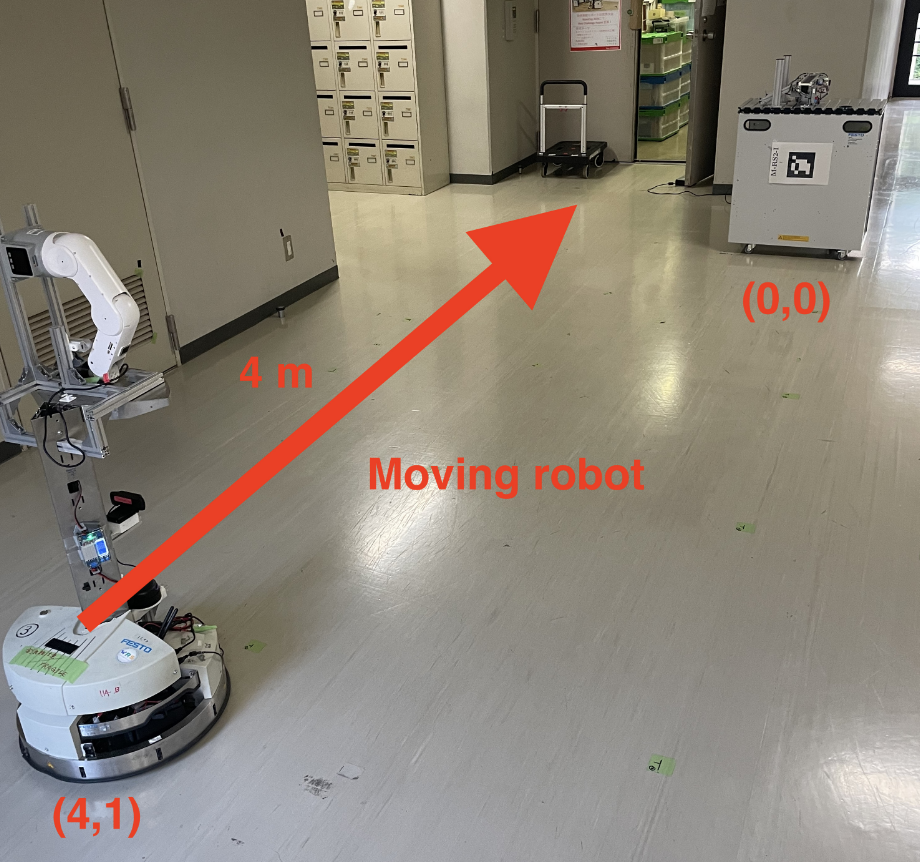
\includegraphics[width=\textwidth]{images/aruco-example-1.png}
        \caption{Robot localisation (\cite{AI-Assisted-Drone-Localization})}
        \label{fig:aruco1}
    \end{subfigure}
    \hfill
    \begin{subfigure}[b]{0.45\textwidth}
        \centering
        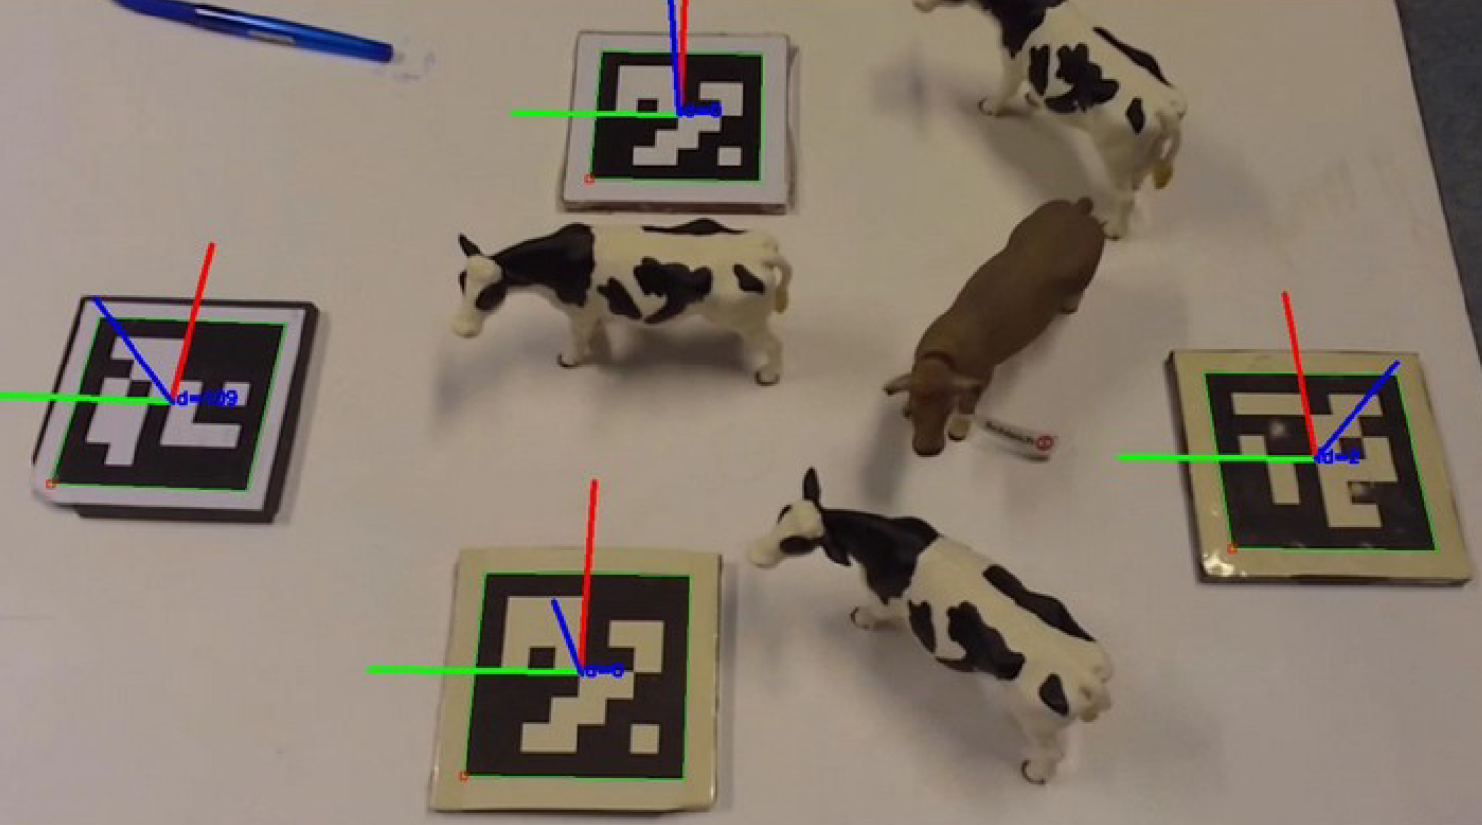
\includegraphics[width=\textwidth]{images/aruco-example-2.png}
        \caption{Drone localisation (\cite{Nakajima2024AboutAE})}
        \label{fig:aruco2}
    \end{subfigure}
    \caption{Examples of ArUco markers in different conditions}
    \label{fig:aruco_markers}
\end{figure}

As \textcite{FiducialMarkerNoisy}, \textcite{ROMERORAMIREZ2021104094}, and others point out, traditional detection methods perform well under controlled 
conditions, but less reliably with real-world challenges, such as rotations, blur and noise. Building on that, this work explores deep learning 
approaches to solve the following challenges:

\begin{enumerate}
  \item Recognising which variation of the marker is present: Classifying ArUco markers under varying blur, noise, and rotation conditions. 
  \item Tracking marker's position in the image: Detecting ArUco markers under varying blur, noise, and rotation conditions. 
\end{enumerate}

\section{Classification}

\subsection{Classification Methodology}

\begin{figure}[h]
  \centering
  \begin{subfigure}[b]{0.2\textwidth}
      \centering
      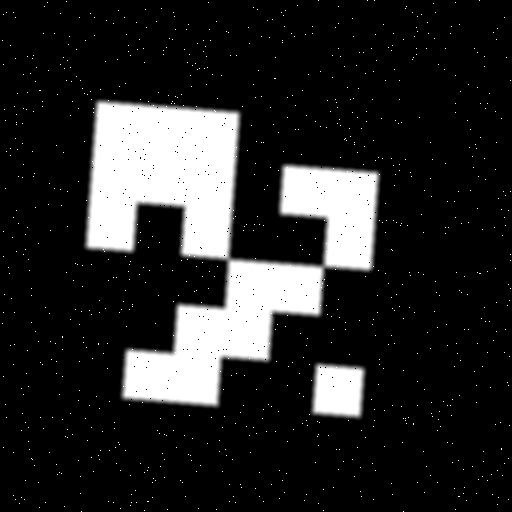
\includegraphics[width=\textwidth]{images/aruco-file3-classification-1.png}
      \caption{Class 0 (out of 100) marker example 1}
      \label{fig:class_ex1}
  \end{subfigure}
  \hfill
  \begin{subfigure}[b]{0.2\textwidth}
      \centering
      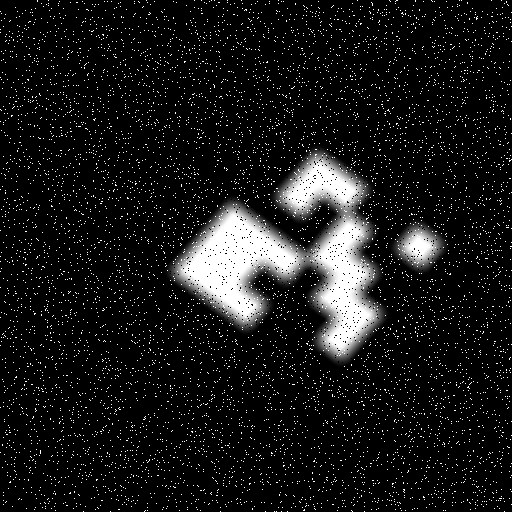
\includegraphics[width=\textwidth]{images/aruco-file3-classification-2.png}
      \caption{Class 0 (out of 100) marker example 2}
      \label{fig:class_ex2}
  \end{subfigure}
  
  \vspace{0.5cm}
  
  \begin{subfigure}[b]{0.2\textwidth}
      \centering
      
\includegraphics[width=\textwidth]{images/aruco-file3-classification-3.png}
      \caption{Class 1 (out of 100) marker example 1}
      \label{fig:class_ex3}
  \end{subfigure}
  \hfill
  \begin{subfigure}[b]{0.2\textwidth}
      \centering
      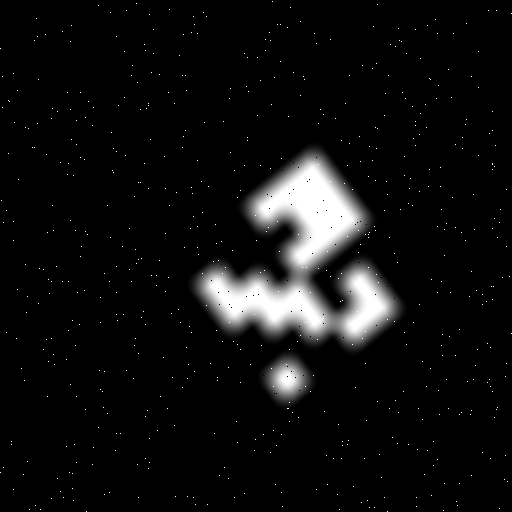
\includegraphics[width=\textwidth]{images/aruco-file3-classification-4.png}
      \caption{Class 1 (out of 100) marker example 2}
      \label{fig:class_ex4}
  \end{subfigure}
  \caption{Examples of ArUco marker classification under different conditions (from the provided dataset)}
  \label{fig:classification_examples}
\end{figure}

The classification dataset examples are visible in figure \ref{fig:classification_examples}.
There are 100 variations/classes of the ArUco marker, and the development of a suitable classification model was broken down into the following steps:

\begin{enumerate}
  \item Create a data plotter for datasets and results
  \item Develop data augmentation script for prepation of a larger dataset  
  \item Prepare classification network architectures
  \item Design experiment to compare classification architectures and parameters
  \item Train and test the final selected classification model
\end{enumerate}

\subsubsection{Data Preparation}

Firstly, the dataset browser was developed. It was initially used to browse the dataset and understand the data. It shows the image,
pixel distribution, and basic dataset statistics.
The idea was that this same tool would later be used to plot the data and results. This can be seen in Figure \ref{fig:data_browser_1}.

\begin{figure}[h]
  \centering
  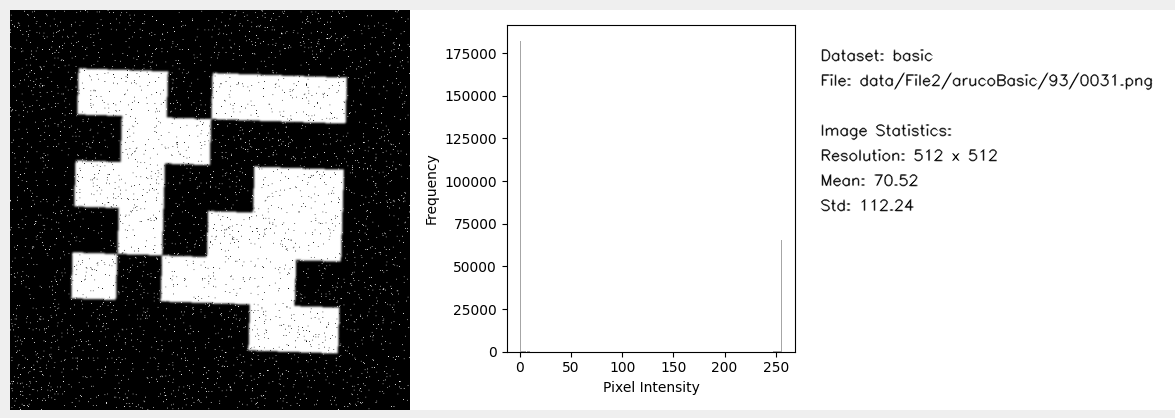
\includegraphics[width=0.45\textwidth]{images/aruco-dataset-browser-1.png}
  \caption{Dataset browser used with the File2 dataset}
  \label{fig:data_browser_1}
\end{figure}

After analysing the data, the data augmentation script was developed. It was used to create a larger dataset for training.
Trial and error was used to find the optimal parameters for the data augmentation that would approximate the augmentations performed
on the data in the dataset provided in File3. With this, the dataset could easily be expanded to include any number of images. The selected
dataset size was 1000 images per class, each image being 512x512 pixels. The data augmentation pipeline uses the raw, unprocessed images in File1, in this file, 
there is a total of 100 images, each is a different variation of the ArUco marker. All of the parameters can be changed in the central configuration file.

The methodology of the data augmentation pipeline is shown below:

\begin{figure}[H]
  \begin{algorithm}[H]
  \caption{Data Augmentation Pipeline}
  \begin{algorithmic}[1]
  \STATE List all of the images in the File1 dataset
  \WHILE{size of augmentations list $<$ target dataset size}
      \STATE Select random rotation, between 0 and 360 degrees
      \STATE Select random scaling, between 50\% and 100\% of original size
      \STATE Select random blur, between 0 and 14 sigma
      \STATE Select random noise, between 0\% and 10\% of pixels
      \STATE Append the set of augmentations to the list
    \ENDWHILE
  \FOR{each image in File1}
      \STATE Create folder named after the image's number (0-99)
      \STATE Read the raw image
      \FOR{each set in the list of augmentations}
        \STATE Apply the augmentations to the image
        \STATE Save the augmented image to the new folder
      \ENDFOR
    \ENDFOR
  \end{algorithmic}
  \end{algorithm}
  \caption{Classification training workflow}
  \end{figure}

\subsubsection{Network Architectures}

Multiple architectures were implemented from the PyTorch library, and tested. To begin with, based on \textcite{pytorch_cifar10}, a simple CNN was implemented to test
how a simple model would perform. Then AlexNet with and without pre-training was implemented to compare the difference. ResNet18 and GoogLeNet were also implemented
from the guidance within the documentation \textcite{pytorch_models}. The modularity of the code allows further model adoption quickly.

Out of many more trialed architectures, the following ones functioned straight out of the box and were used in the initial experiment:

\begin{itemize}
    \item \textbf{MinimalCNN}: A lightweight custom architecture with:
    \begin{itemize}
        \item Three convolutional blocks (32$\rightarrow$64$\rightarrow$128 features)
        \item Batch normalisation and dropout for regularisation
        \item Global average pooling for dimension reduction
    \end{itemize}
    
    \item \textbf{AlexNet Variants}:
    \begin{itemize}
        \item Clean implementation without pre-training
        \item Version with pre-trained features
    \end{itemize}
    
    \item \textbf{ResNet18}: Pre-trained implementation
    \item \textbf{GoogLeNet}: Pre-trained implementation
\end{itemize}

\subsubsection{Training Configuration}

Combinations of all of the selected networks, and all of the following additional parameters were trained:

\begin{itemize}
  \item \textbf{Datasets}: File3 (provided dataset with 100 images in all of the 100 provided classes, strong distortions)
  \item \textbf{Models}: MinimalCNN, AlexNet-clean, AlexNet, ResNet18, GoogLeNet
  \item \textbf{Batch Sizes}: 32, 64
  \item \textbf{Additional Random Training Transformations}: None, random rotations, random rotation blur and noise
\end{itemize}

These experiment parameters form 30 different combinations, thus 30 different networks and sets of results, with training time on a single GPU for total of nearly 8 hours. 
With a single change in the configuration file, the entire experiment can be changed, the custom dataset (or more datasets) can be used (increasing time per epoch), different
batch sizes can be used (increasing memory usage beyond the used GPU's capability), different transformations can be used, and different models can be used.

Additional settings and parameters purely for the purpose of limiting the time to run the experiment were used:

\begin{itemize}
    \item \textbf{Loss Function}: Cross-entropy
    \item \textbf{Optimizer}: Adam with learning rate 3e-4
    \item \textbf{Training Duration}: 50 epochs with early stopping at 96\% training accuracy 
\end{itemize}

After the experiments were completed, the results were plotted and analysed. The results are shown in the following section, and full results are available in the results directory
and the appendices.

The final model was trained on the custom dataset, with the following parameters and settings derived based on the best performing combination of the initial experiments:

\begin{itemize}
  \item \textbf{Datasets}: Custom dataset (1000 images per class)
  \item \textbf{Model}: GoogLeNet
  \item \textbf{Batch Sizes}: 32
  \item \textbf{Additional Random Training Transformations}: None
\end{itemize}

\subsubsection{Method Implementation}

The experiment implementation followed this algorithmic workflow:

\begin{figure}[H]
\begin{algorithm}[H]
\caption{Classification Experiment Pipeline}
\begin{algorithmic}[1]
\STATE Load configuration for dataset, model, batch size, and transformations
\FOR{each combination in configurations}
    \STATE Load dataset
    \STATE Setup results directory
    \STATE Initialise model and transforms
    \STATE Create data loaders
    \STATE Initialise loss function, optimiser
    \STATE Train and validate model for number of epochs
    \STATE Plot the training progress
    \STATE Run evaluation on test set
    \STATE Plot classification metrics
    \STATE Save all results
\ENDFOR
\end{algorithmic}
\end{algorithm}
\caption{Classification experiment workflow}
\end{figure}

The model training loop is shown below:

\begin{figure}[H]
\begin{algorithm}[H]
\caption{Classification Training and Validation Pipeline}
\begin{algorithmic}[1]
\FOR{each epoch in total number of epochs}
    \STATE Set model to train mode
    \FOR{each batch in train loader}
        \STATE Reset gradients
        \STATE Forward pass through network
        \STATE Calculate cross-entropy loss
        \STATE Backpropagate and update weights
        \STATE Add loss and accuracy to totals
    \ENDFOR
    \STATE Calculate average training loss and accuracy
    \STATE Set model to evaluation mode
    \FOR{each batch in validation loader}
        \STATE Forward pass through network
        \STATE Calculate cross-entropy loss
        \STATE Add loss and accuracy to totals
    \ENDFOR
    \STATE Calculate average validation loss and accuracy
    \STATE Save model if the best validation accuracy was achieved
    \STATE Check for early stopping criteria
\ENDFOR
\end{algorithmic}
\end{algorithm}
\caption{Classification training workflow}
\end{figure}

The final training loop reused most of the code from the above. The only change was that
after successful training on the custom dataset, the model was loaded again, and the two original
datasets were used to create test only dataloaders and the model was tested on them individually.

\subsection{Classification Results}

The classification experiments were conducted in two phases. Initially, multiple architectures
and configurations were tested on the File3 dataset to determine the optimal approach. Subsequently, the best
performing configuration was trained on a custom dataset and evaluated against both File2 and File3.

\subsubsection{Initial Experiments}

The experiments encompassed various architectures with different batch sizes and data augmentation strategies. Each
configuration was tested on 1000 samples from File3, with the following results:

\begin{itemize}
    \item \textbf{MinimalCNN}:
        \begin{itemize}
            \item Batch size 32, full (training time) augmentation: 5.20\% accuracy (F1: 3.62\%)
        \end{itemize}

    \item \textbf{AlexNet (Clean Implementation)}:
        \begin{itemize}
            \item Batch size 64, rotation (training time) augmentation: 98.60\% accuracy (F1: 98.51\%)
        \end{itemize}
    
    \item \textbf{AlexNet (Pre-trained)}:
        \begin{itemize}
            \item Batch size 64, full (training time) augmentation: 73.70\% accuracy (F1: 72.15\%)
        \end{itemize}
    
    \item \textbf{ResNet18}:
        \begin{itemize}
            \item Batch size 32, no (training time) augmentation: 100.00\% accuracy (F1: 100.00\%)
        \end{itemize}
    
    \item \textbf{GoogLeNet}:
        \begin{itemize}
            \item Batch size 32, no (training time) augmentation: 99.90\% accuracy (F1: 99.87\%)
        \end{itemize}
\end{itemize}

The experiment results are shown in the figure \ref{fig:training_progress}.

\begin{figure}[h]
    \centering
    \begin{subfigure}[b]{0.45\textwidth}
      \centering
      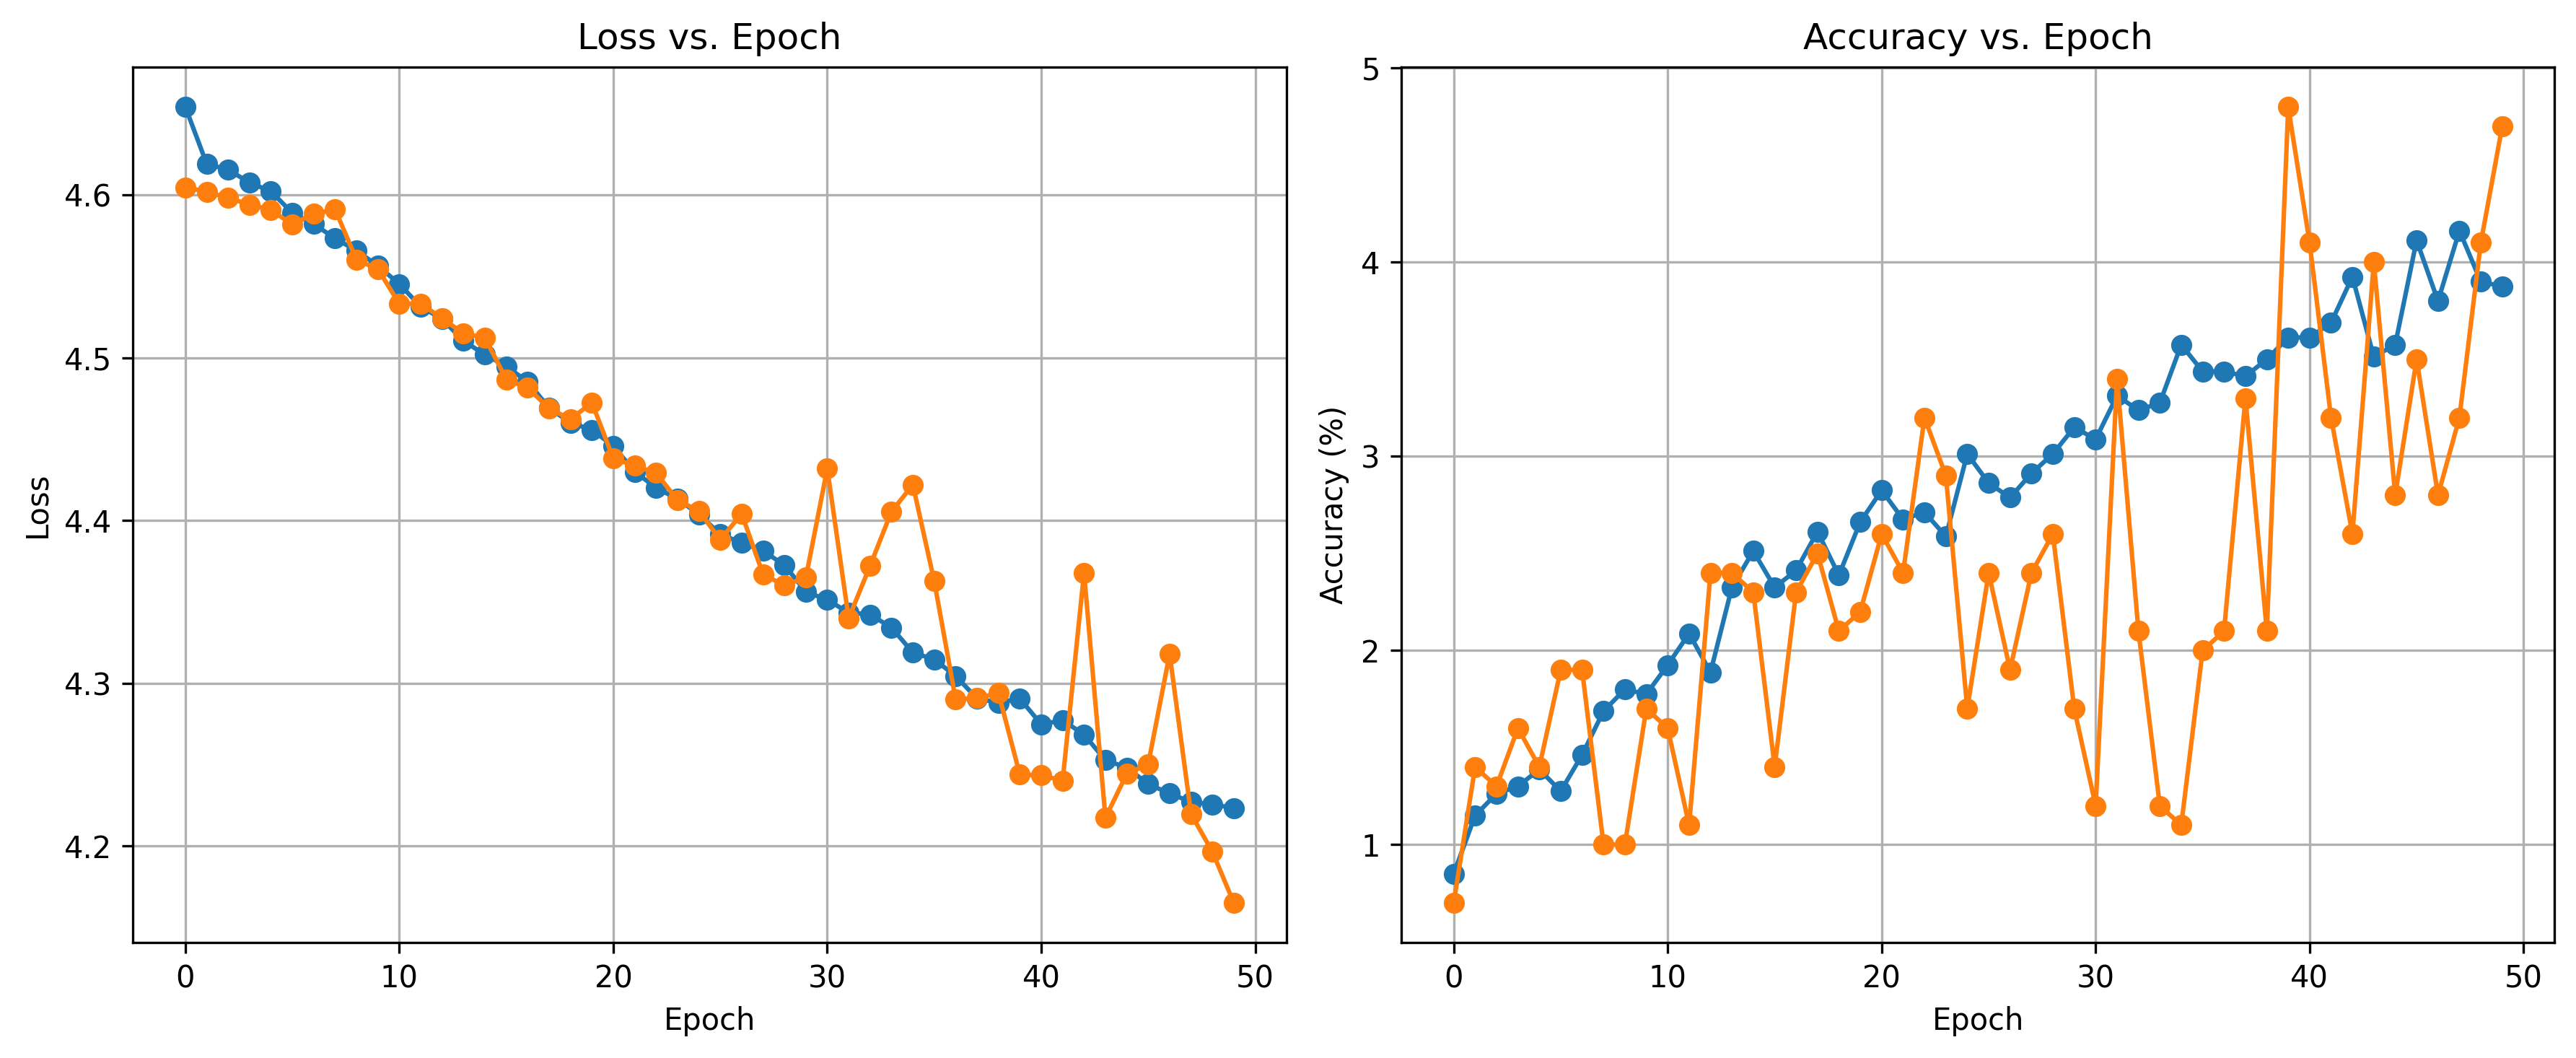
\includegraphics[width=\textwidth]{images/training_progress_MinimalCNN.png}
      \caption{MinimalCNN training progress}
      \label{fig:progress_minimalcnn}
    \end{subfigure}
    \hfill
    \begin{subfigure}[b]{0.45\textwidth}
      \centering
      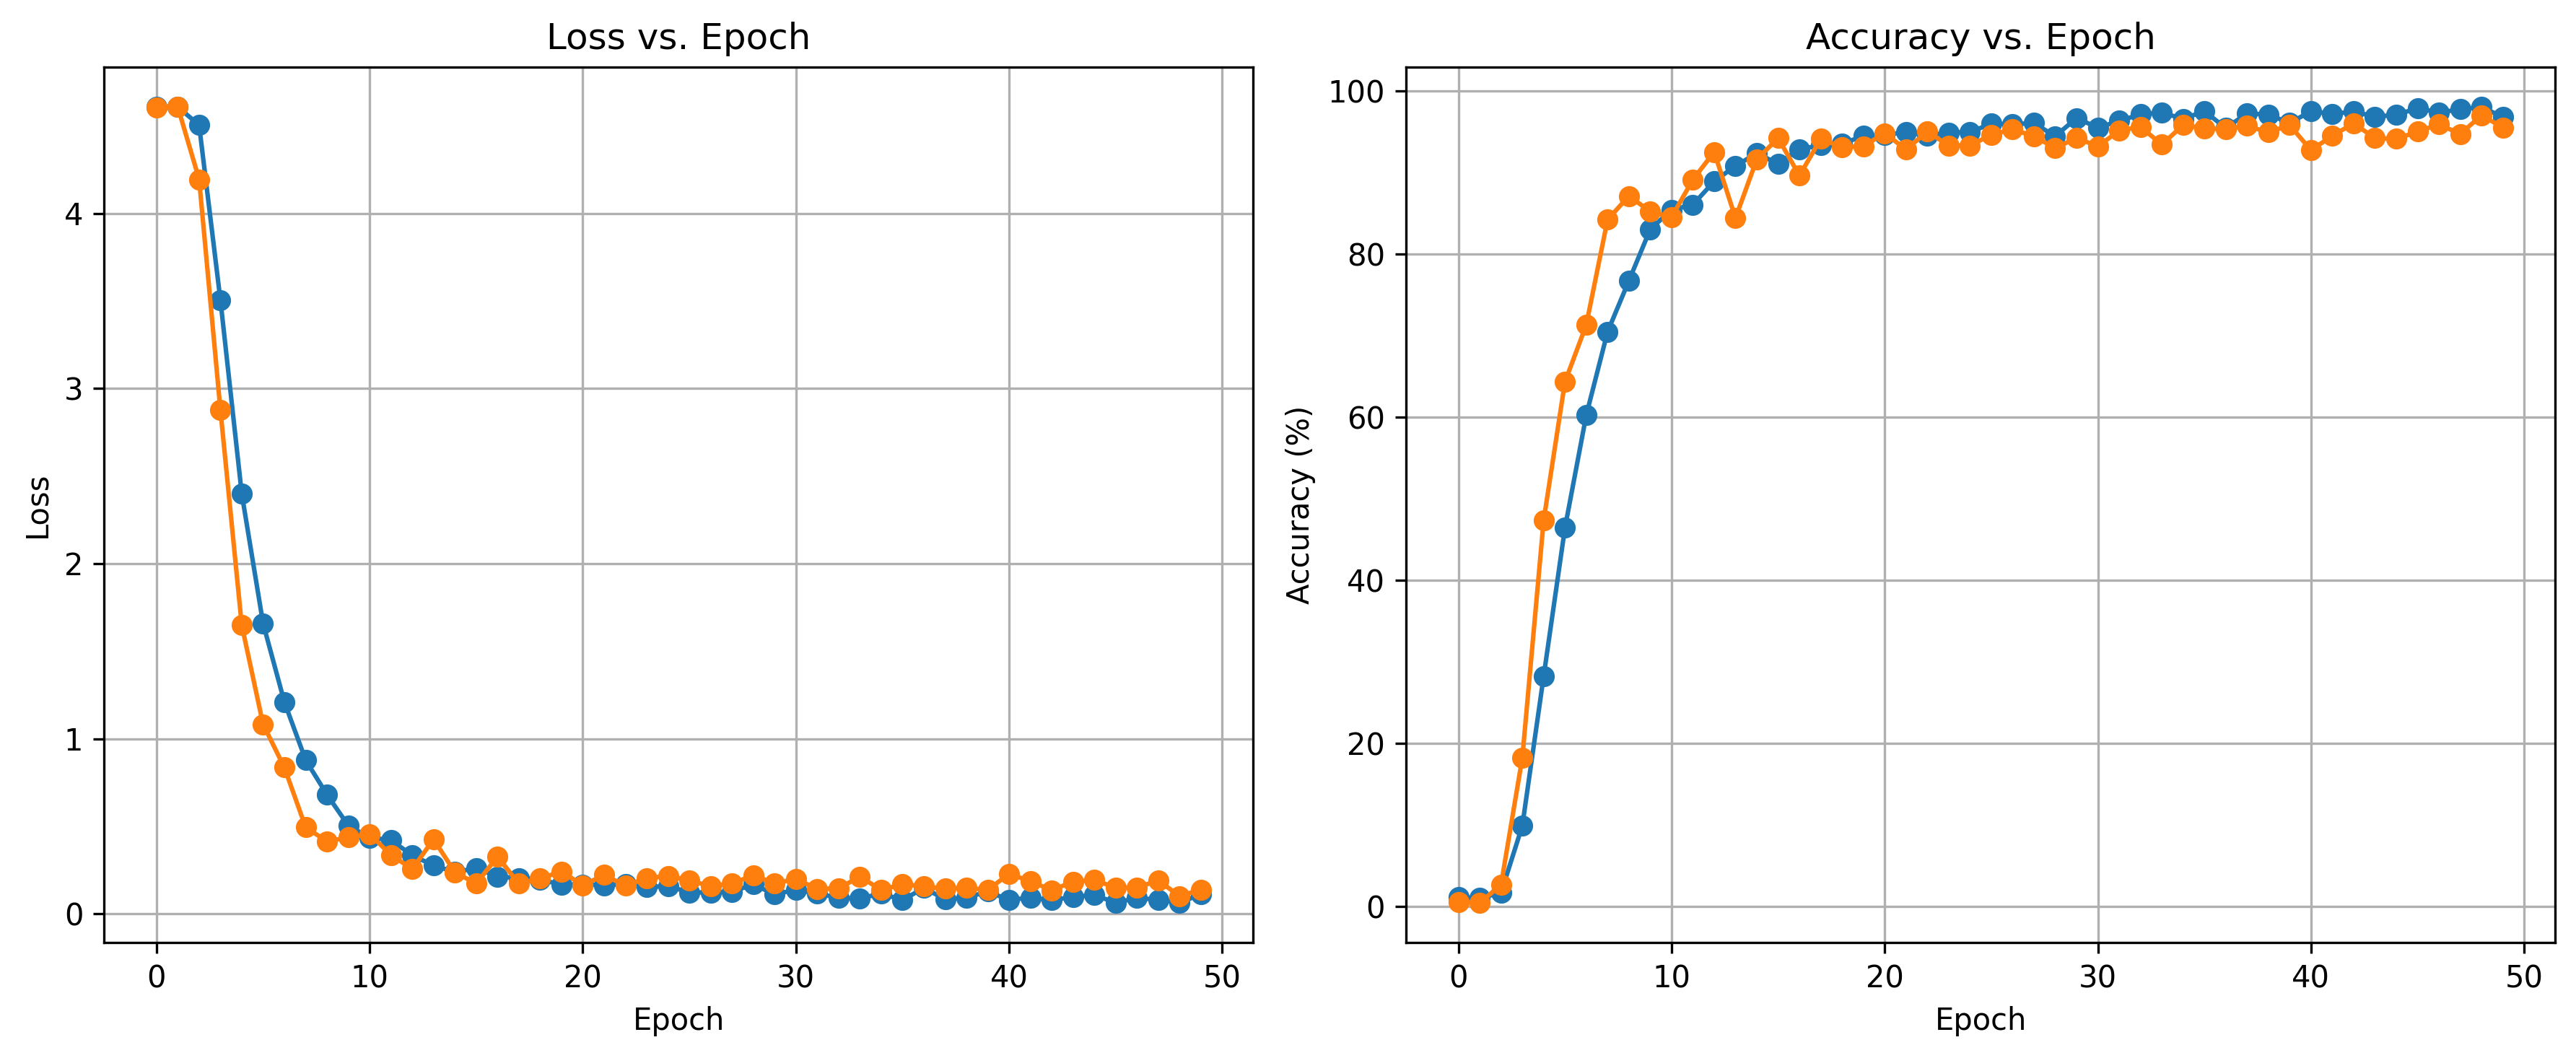
\includegraphics[width=\textwidth]{images/training_progress_AlexNet_clean.png}
      \caption{AlexNet (clean) training progress}
      \label{fig:progress_alexnet_clean}
    \end{subfigure}    
    \vspace{0.5cm}
    \begin{subfigure}[b]{0.45\textwidth}
      \centering
      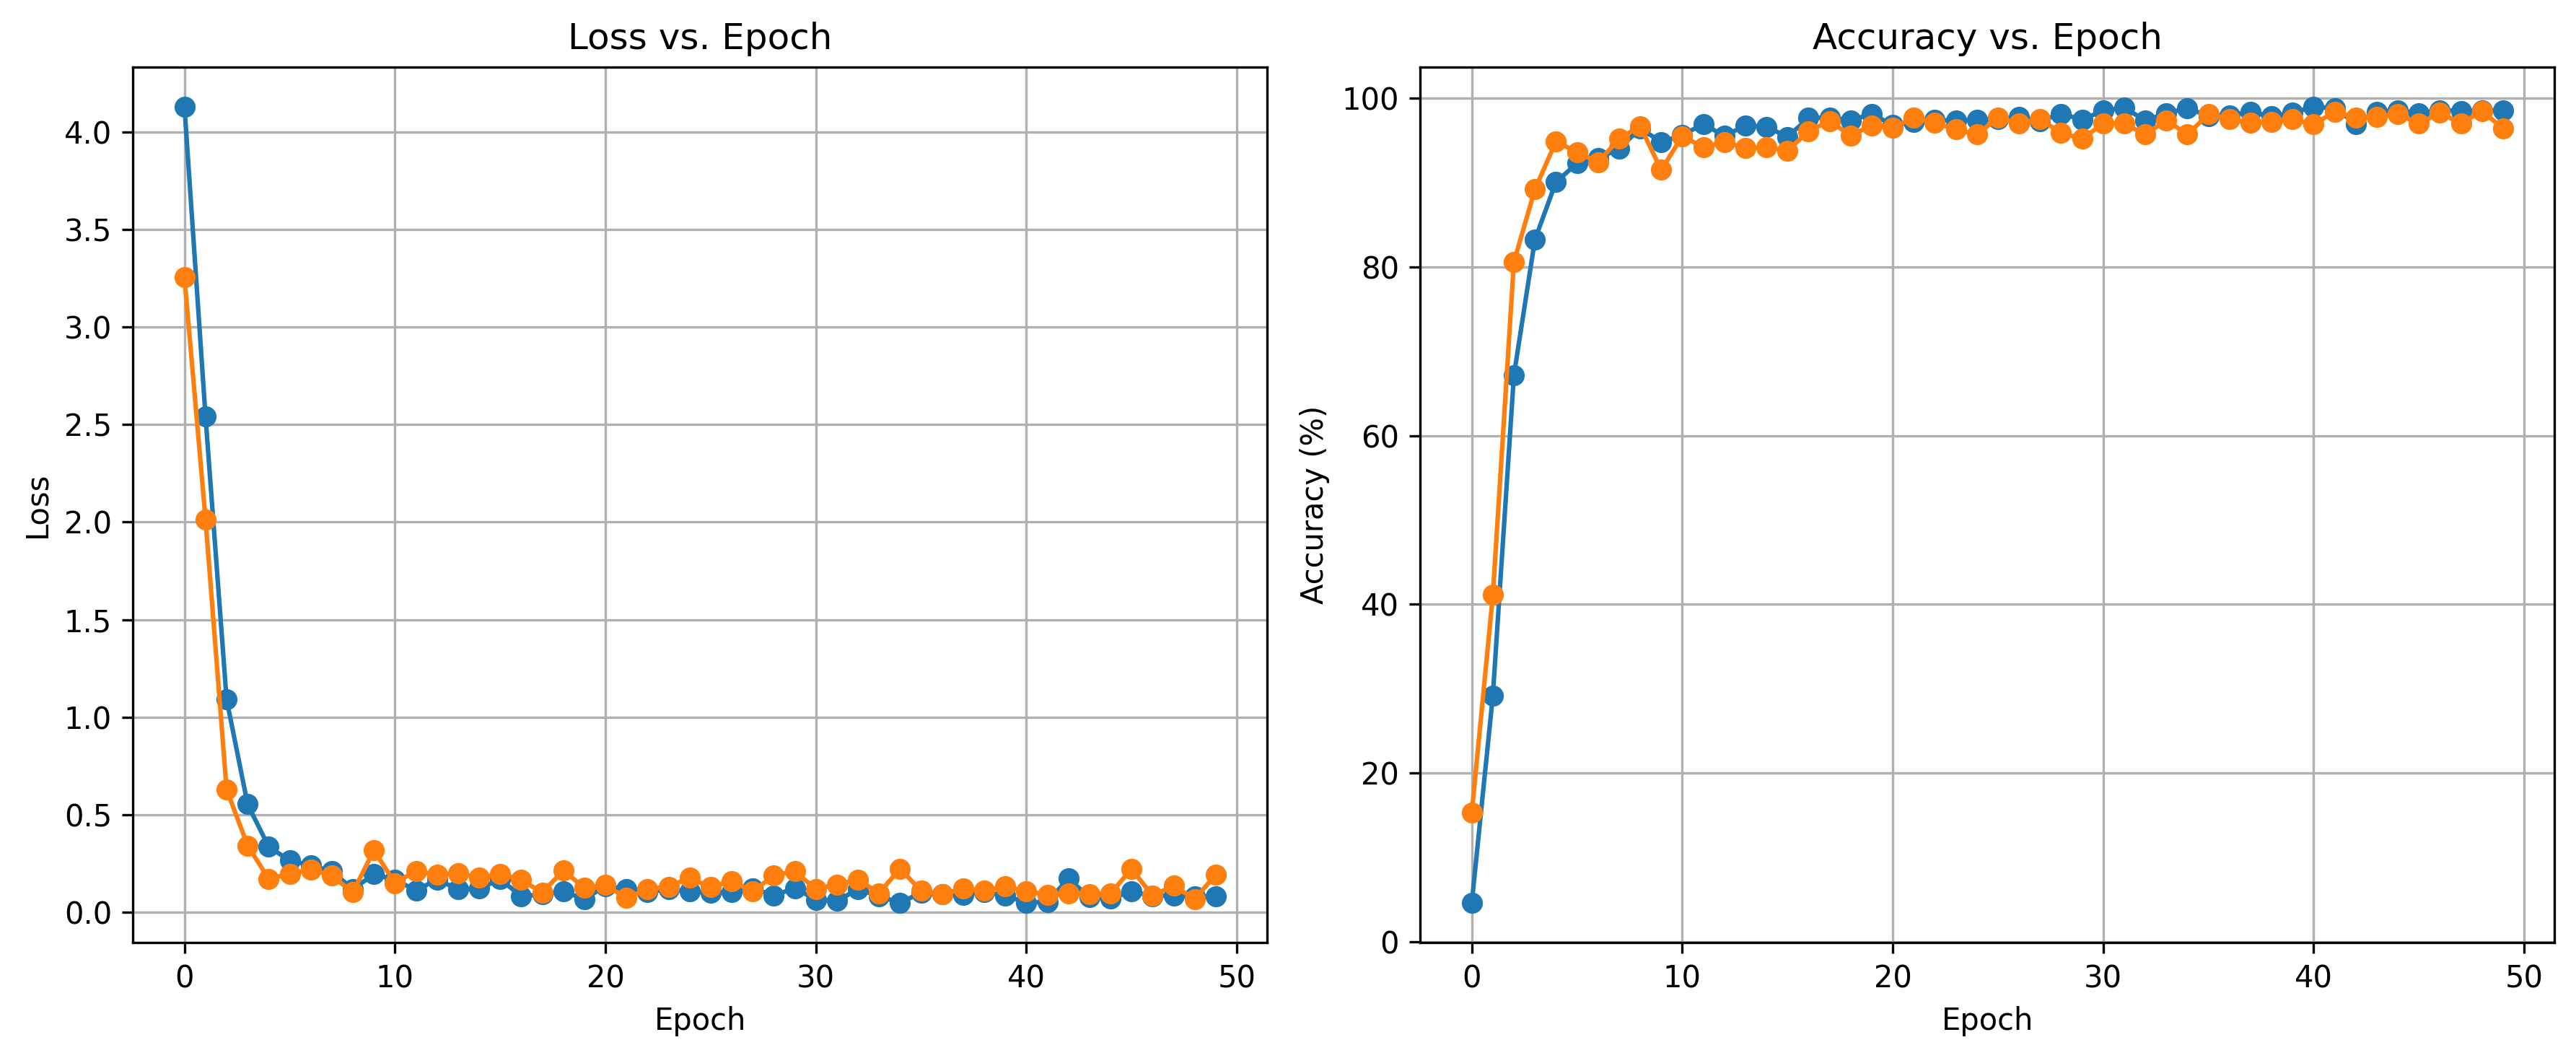
\includegraphics[width=\textwidth]{images/training_progress_AlexNet.png}
      \caption{AlexNet (pre-trained) training progress}
      \label{fig:progress_alexnet}
    \end{subfigure}
    \hfill
    \begin{subfigure}[b]{0.45\textwidth}
        \centering
        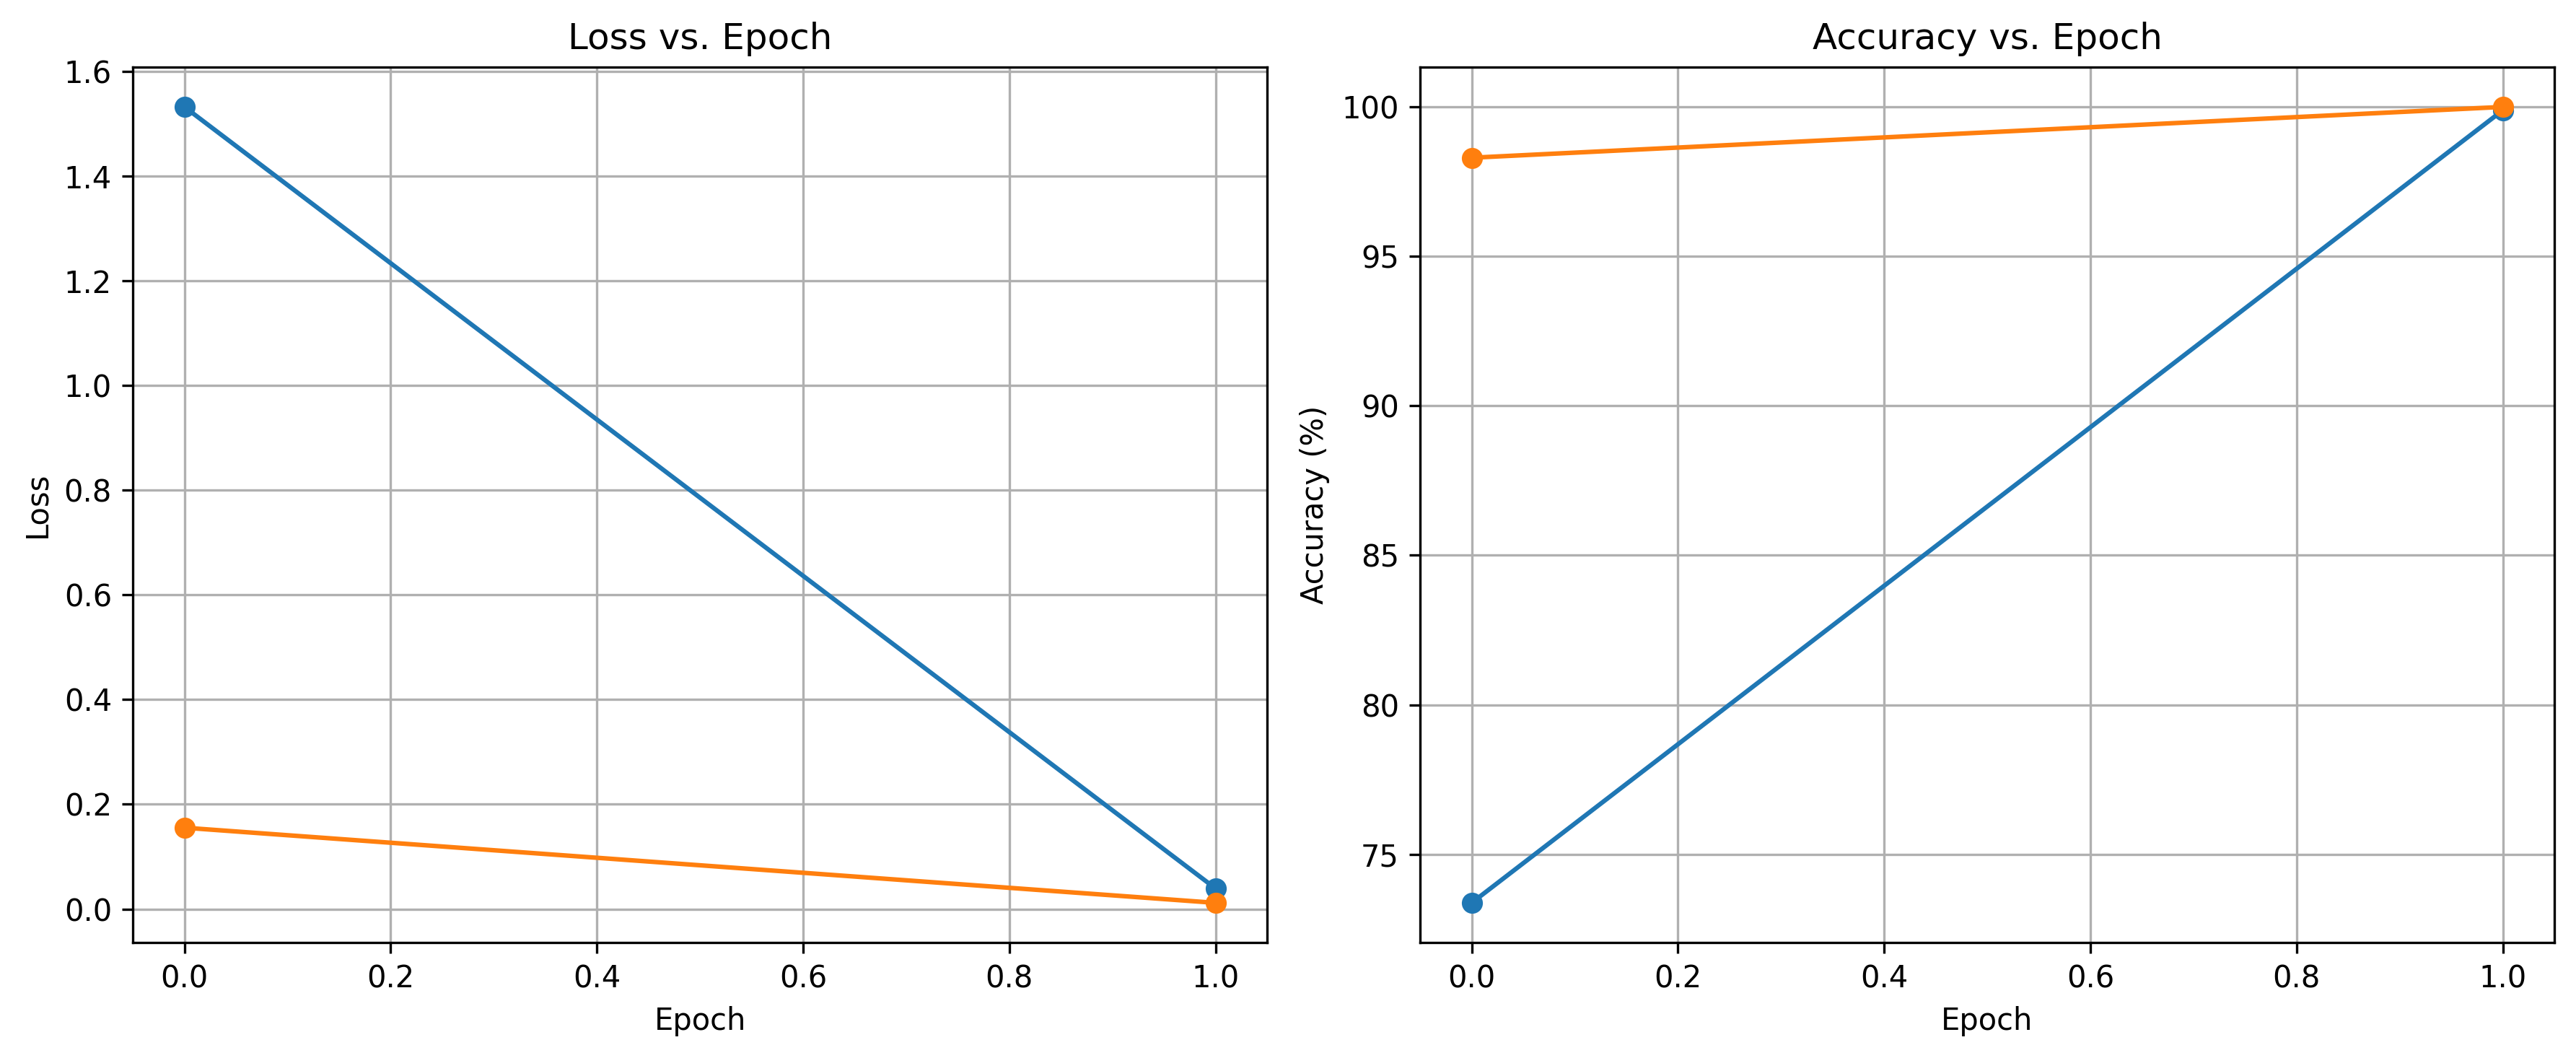
\includegraphics[width=\textwidth]{images/training_progress_ResNet.png}
        \caption{ResNet18 training progress}
        \label{fig:progress_resnet}
    \end{subfigure}
    \caption{Training progress for different model architectures showing training and validation accuracy over epochs (orange plot is validation accuracy,
    blue is training accuracy)}
    \label{fig:training_progress}
\end{figure}

All of the training progress plots show the training progress of the models with 32 batch size and no data augmentation for comparability.
The results of the minimal CNN are as expected, although the model was indeed training and given many more epochs, it would likely achieve better results.  

As expected, the AlexNet with no pre-trained weights performed very well, but converged much slower than it's pre-trained counterpart.
ResNet18 and GoogLeNet preformed near perfectly, noticebly better without additional training transforms than with them. Only the ResNet's plot
is shown as their are nearly the same. These two models triggered early stopping after reaching 99\% validation accuracy.

For further insights, training logs and detailed analysis, additional plots, results, and data can be found in the Appendices.

\subsubsection{Final Model Performance}

Based on the previous findings, GoogLeNet was selected for the final model due to its consistent performance across different parameter settings.
The model was trained on FileCustom1, a synthetic dataset created to approximate the conditions in Files 2 and 3. This means that the training
data increased from 9,000 samples to 95,000 samples.

The final evaluation yielded these results:

\begin{itemize}
    \item \textbf{Training Evaluation} (2,500 samples):
        \begin{itemize}
            \item Accuracy: 100.00\%
            \item Precision: 100.00\%
            \item Recall: 100.00\%
            \item F1-score: 100.00\%
        \end{itemize}
    \item \textbf{File2 Evaluation} (10,000 samples):
        \begin{itemize}
            \item Accuracy: 100.00\%
            \item Precision: 100.00\%
            \item Recall: 100.00\%
            \item F1-score: 100.00\%
        \end{itemize}
    \item \textbf{File3 Evaluation} (10,000 samples):
        \begin{itemize}
            \item Accuracy: 97.48\%
            \item Precision: 97.68\%
            \item Recall: 97.48\%
            \item F1-score: 97.51\%
        \end{itemize}
\end{itemize}

These results demonstrate the model's near-perfect performance (as shown in figure \ref{fig:final_analysis}) across different distortion conditions.
The perfect scores on File2 indicate excellent handling of weak distortions, while the very good performance on File3
(misclassifying only 252 out of 10,000 samples) shows good resilience to more challenging conditions. Based on the accuracy, precision, and recall
plots per class, we can clearly see that the model fails to identify marker 33 the most as that's where it's precision is the lowest,
whilst markers 14 and 39 are the most frequently missed ones due to the lowest recall. This can be better visualised in the confusion matrix (this can be seen in
the appendices).

\begin{figure}[h]
    \centering
    \begin{subfigure}[b]{0.45\textwidth}
        \centering
        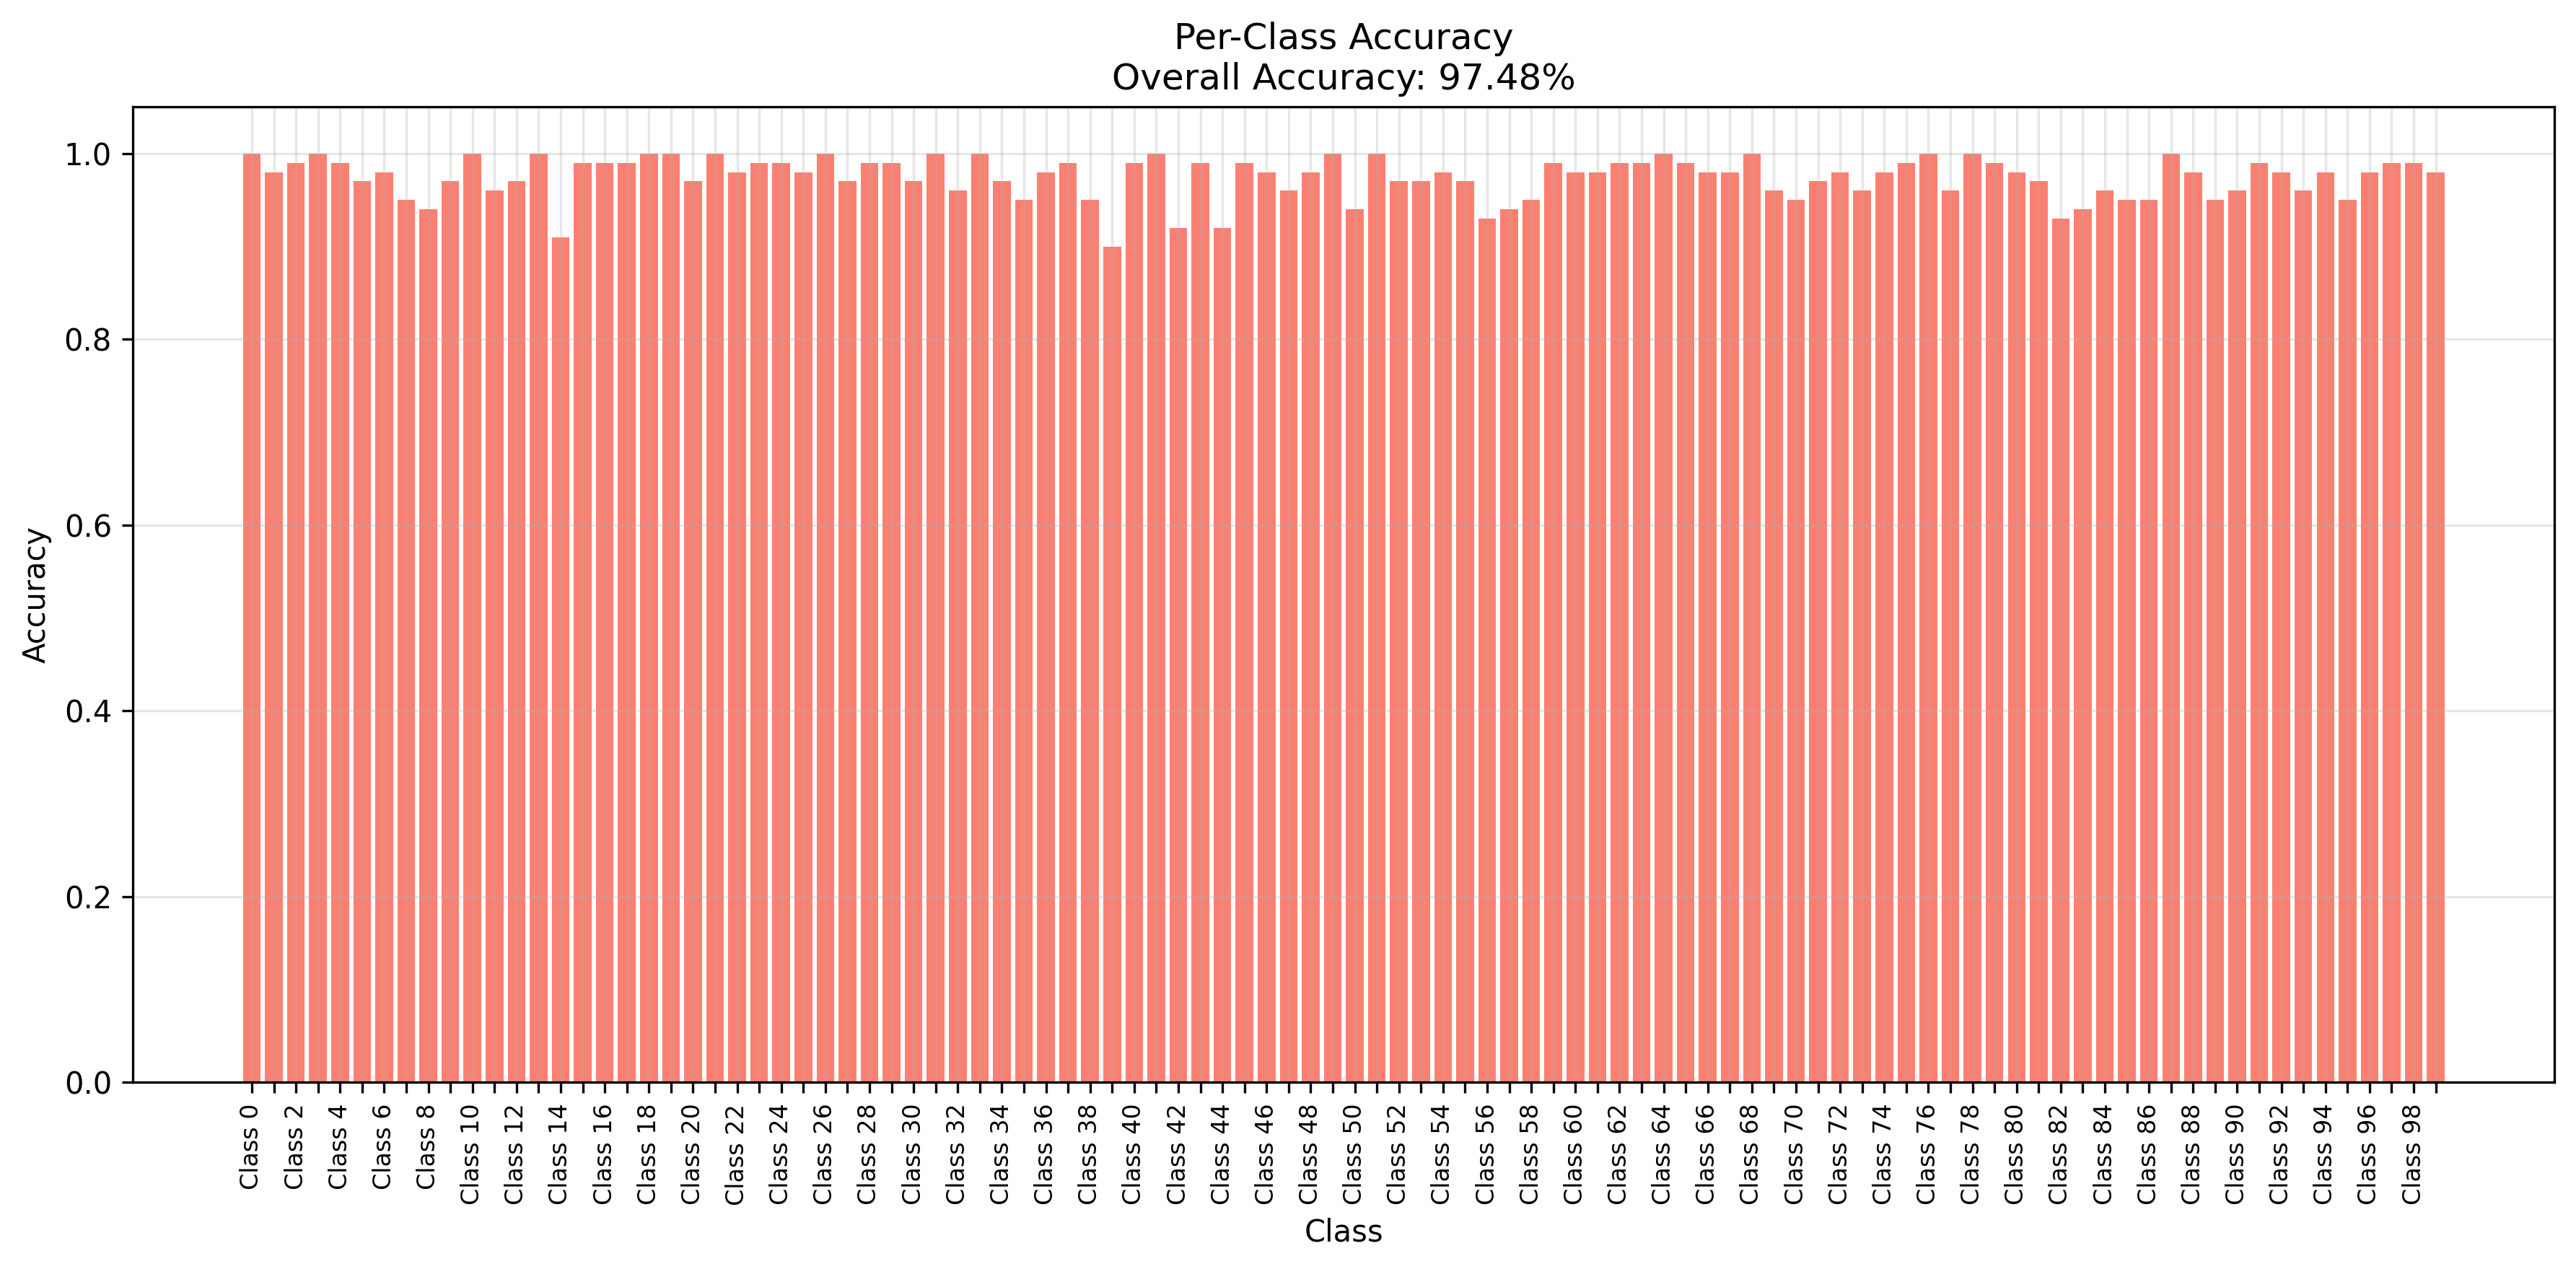
\includegraphics[width=\textwidth]{images/File3_final_analysis_accuracy.png}
        \caption{Per-class accuracy analysis}
        \label{fig:final_accuracy}
    \end{subfigure}
    \hfill
    \begin{subfigure}[b]{0.45\textwidth}
        \centering
        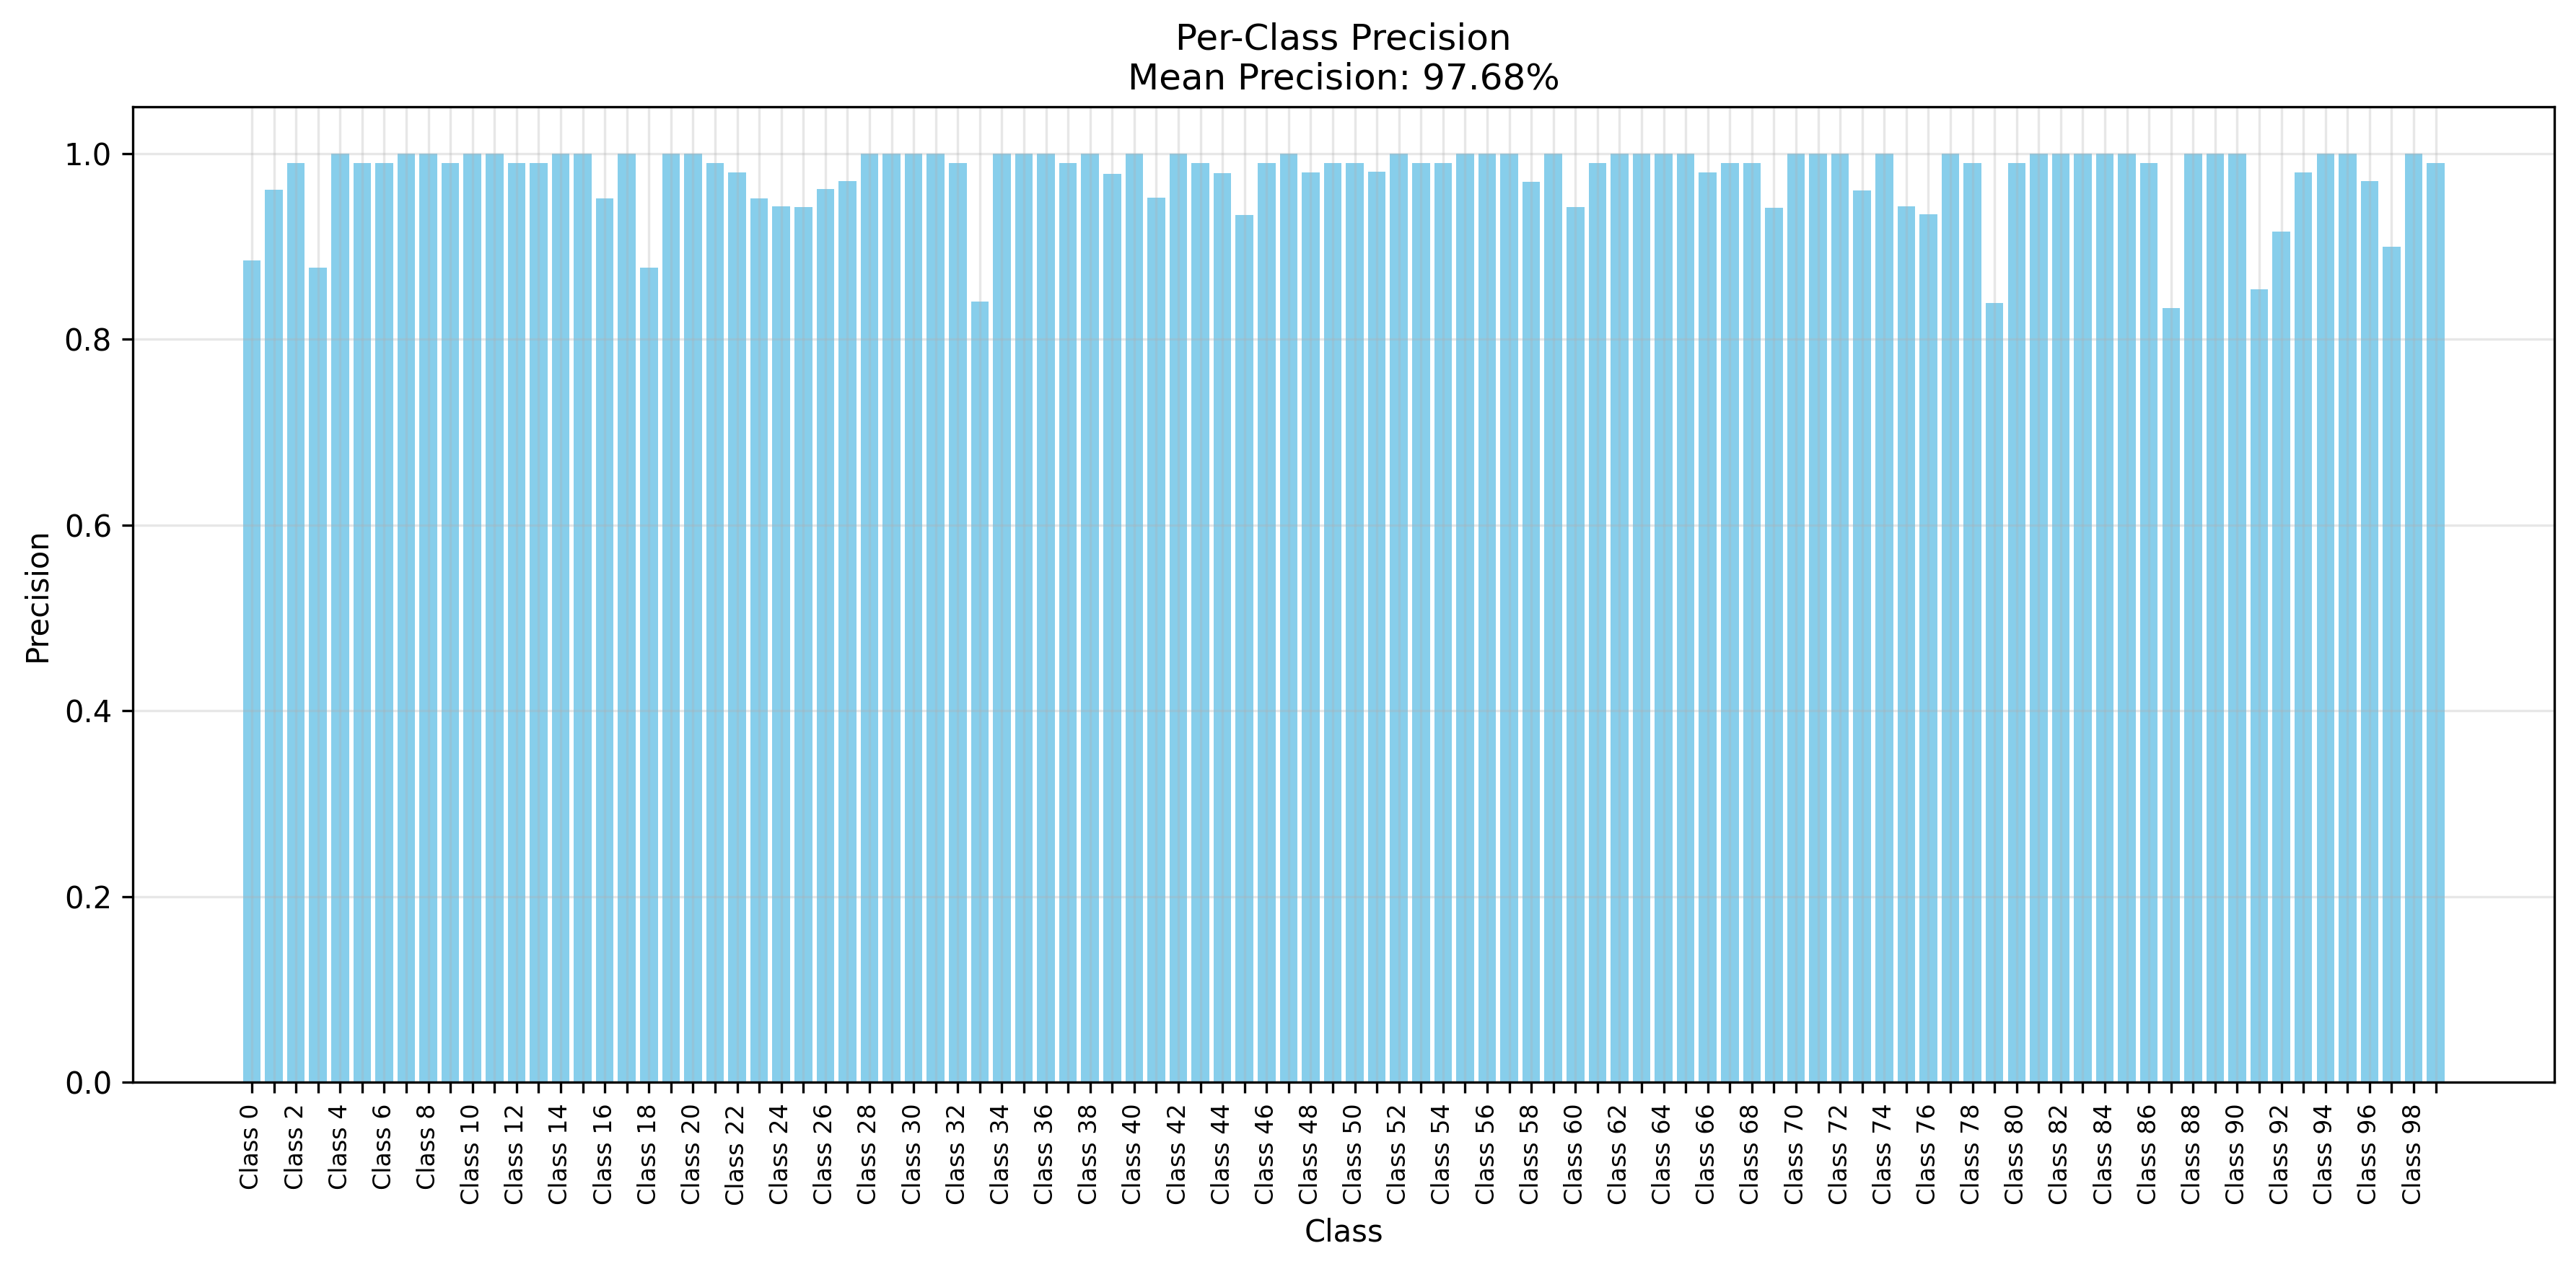
\includegraphics[width=\textwidth]{images/File3_final_analysis_precision.png}
        \caption{Per-class precision analysis}
        \label{fig:final_precision}
    \end{subfigure}
    
    \vspace{0.5cm}
    
    \begin{subfigure}[b]{0.45\textwidth}
        \centering
        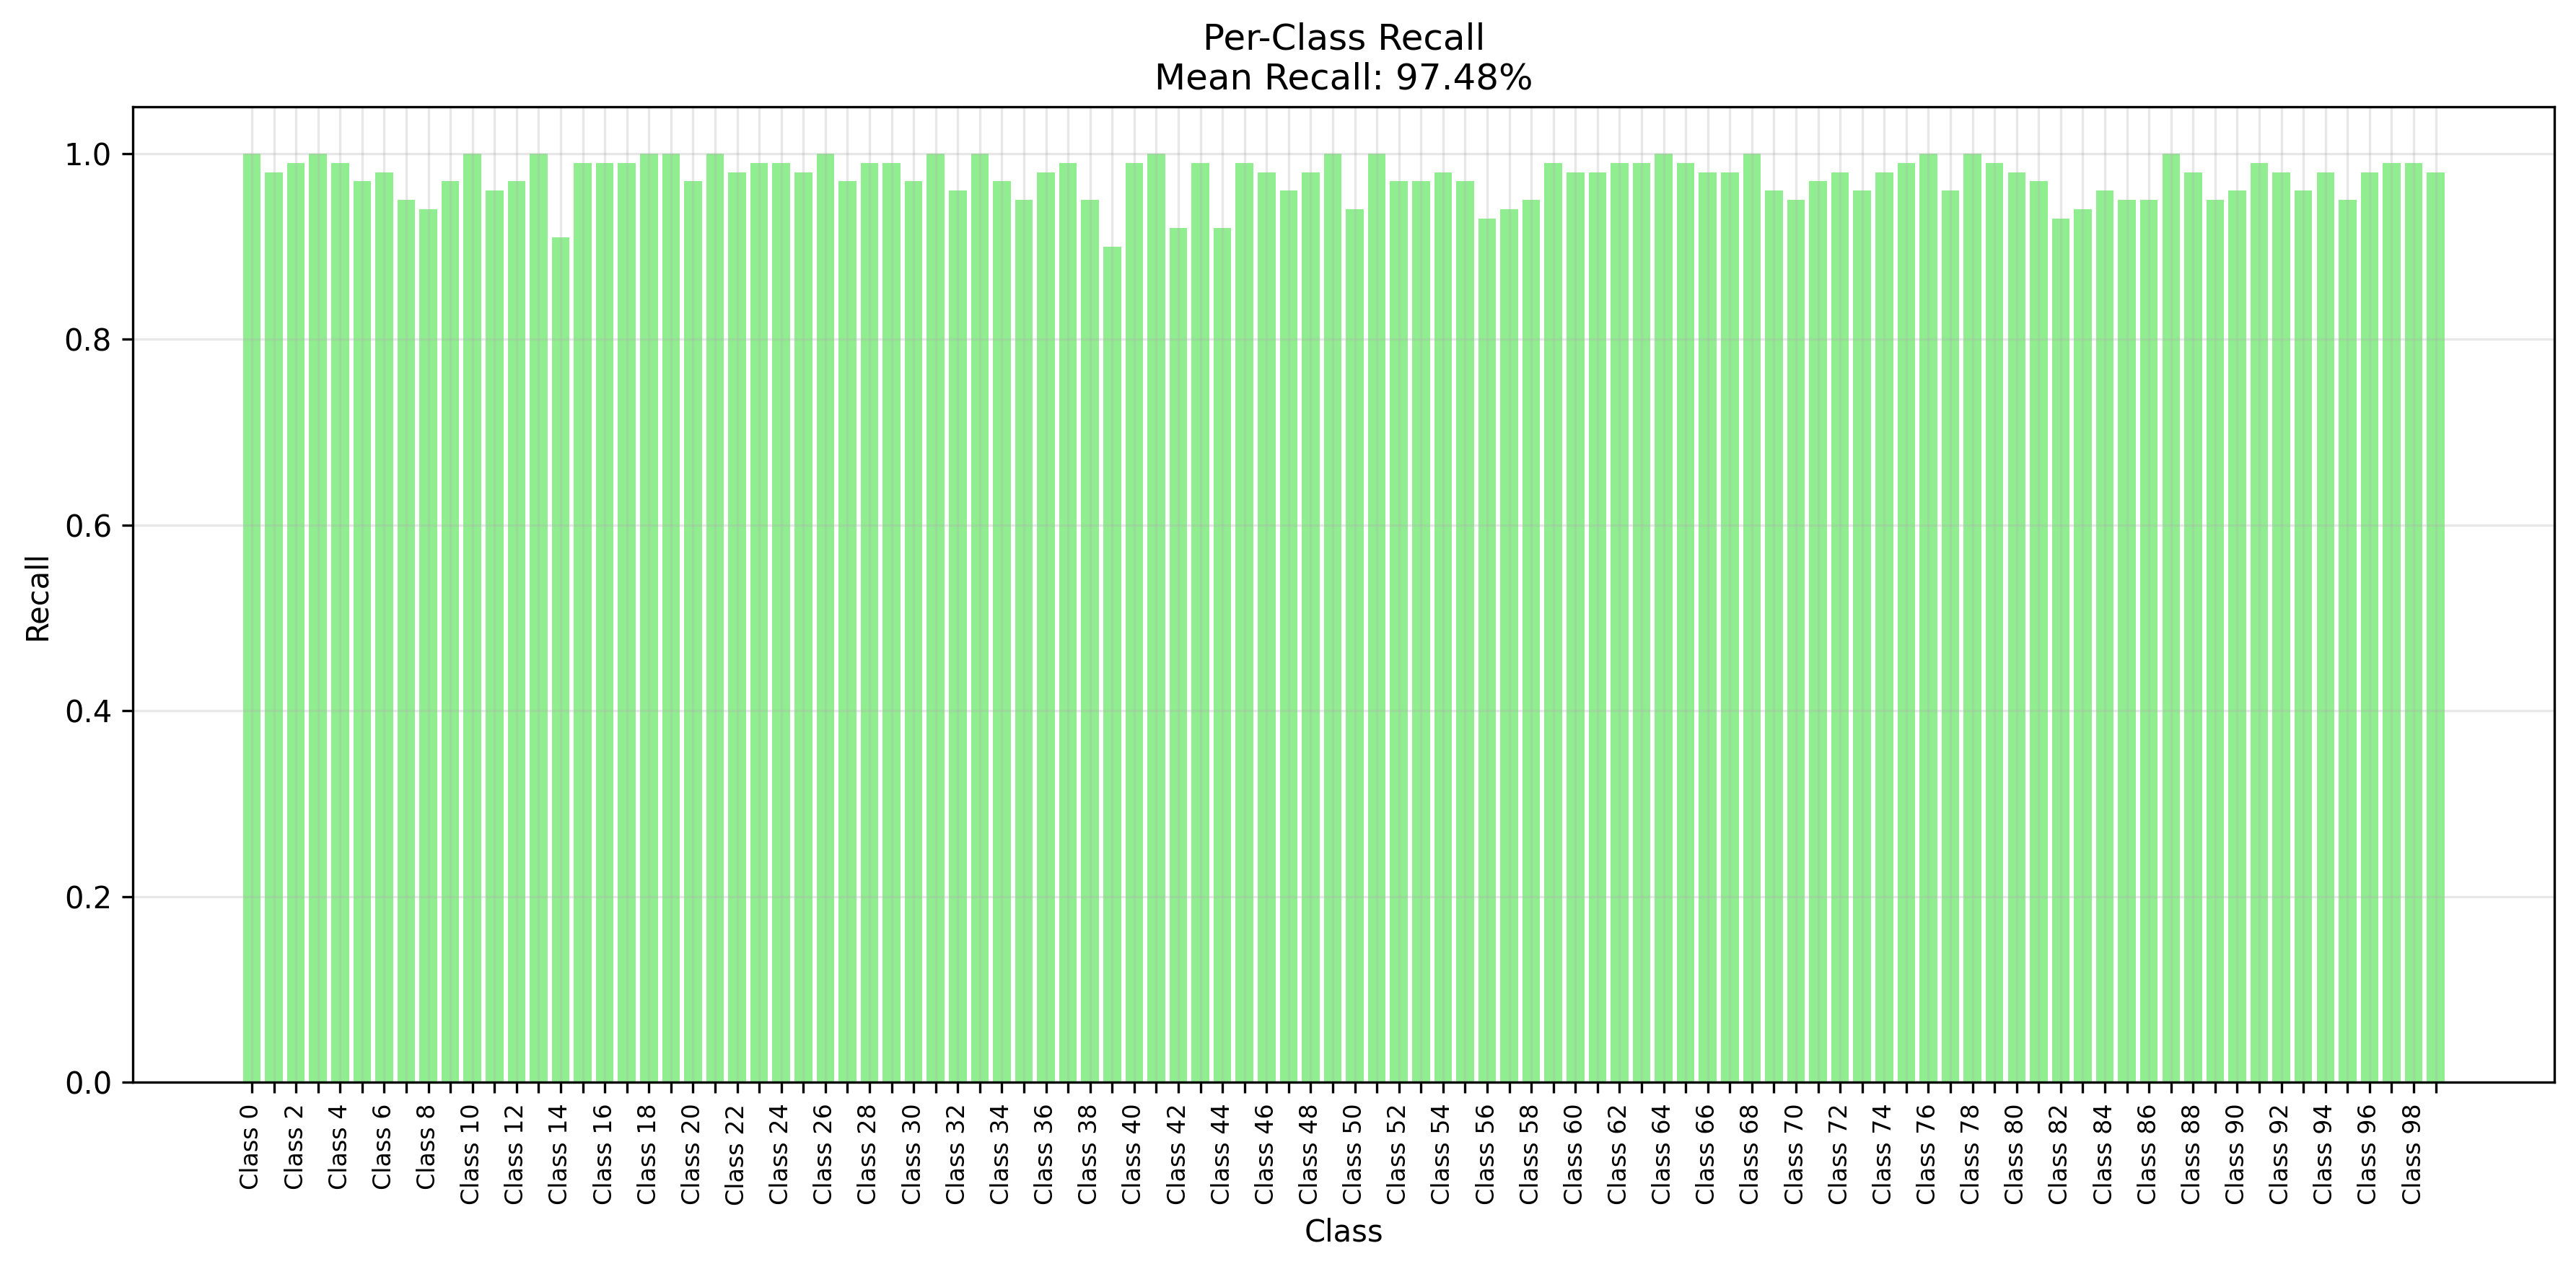
\includegraphics[width=\textwidth]{images/File3_final_analysis_recall.png}
        \caption{Per-class recall analysis}
        \label{fig:final_recall}
    \end{subfigure}
    \caption{Final model performance analysis on File3 dataset showing per-class metrics}
    \label{fig:final_analysis}
\end{figure}

\section{Detection}

\subsection{Detection Methodology}

\begin{figure}[h]
  \centering
  \begin{subfigure}[b]{0.2\textwidth}
      \centering
      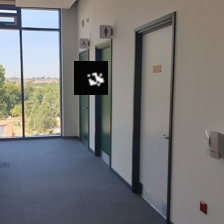
\includegraphics[width=\textwidth]{images/aruco-file4-detection-1.png}
      \caption{Marker in office placement example 1}
      \label{fig:det_ex_1}
  \end{subfigure}
  \hfill
  \begin{subfigure}[b]{0.2\textwidth}
      \centering
      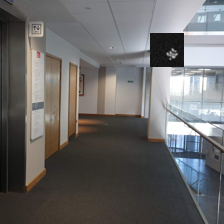
\includegraphics[width=\textwidth]{images/aruco-file4-detection-2.png}
      \caption{Marker in office placement example 2}
      \label{fig:det_ex_2}
  \end{subfigure}
  
  \vspace{0.5cm}
  
  \begin{subfigure}[b]{0.2\textwidth}
      \centering
      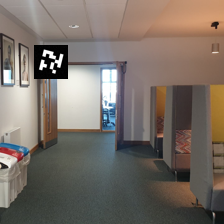
\includegraphics[width=\textwidth]{images/aruco-file4-detection-3.png}
      \caption{Marker in office placement example 3}
      \label{fig:det_ex_3}
  \end{subfigure}
  \hfill
  \begin{subfigure}[b]{0.2\textwidth}
      \centering
      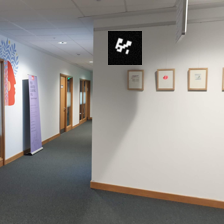
\includegraphics[width=\textwidth]{images/aruco-file4-detection-4.png}
      \caption{Marker in office placement example 4}
      \label{fig:det_ex_4}
  \end{subfigure}
  \caption{Examples of ArUco marker placements (from the provided dataset)}
  \label{fig:detection_examples}
\end{figure}

The detection dataset examples are visible in figure \ref{fig:detection_examples}.
There are 100 examples of the ArUco marker placement and a CSV file with the position of the marker in each one of them.

The detection problem was approached in a similar way to classification, with the following key steps:

\begin{enumerate}
  \item Adapt and prepare the data plotter for detection datasets and results
  \item Develop data augmentation script for office images with ArUco markers
  \item Prepare detection network architectures
  \item Design experiment to compare detection architectures and settings
  \item Train and test the final detection model
\end{enumerate}

\subsubsection{Data Preparation}

Firstly, the dataset browser was asdapted to handle detection data viewing (and results).
It shows the image, it's bounding box (ground truth and prediction if available), pixel distribution, and basic dataset statistics.
This can be seen in Figure \ref{fig:data_browser_2}.

\begin{figure}[h]
  \centering
  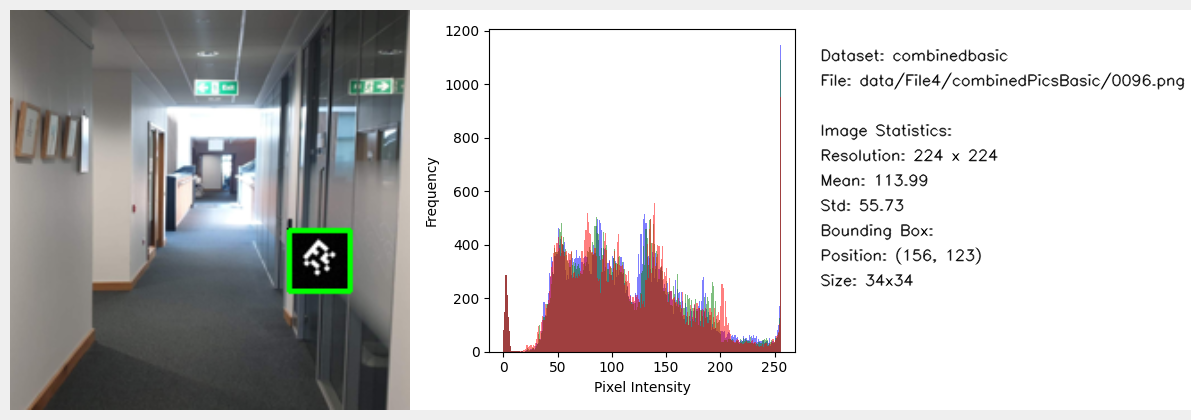
\includegraphics[width=0.45\textwidth]{images/aruco-dataset-browser-2.png}
  \caption{Dataset browser used with the File4 dataset}
  \label{fig:data_browser_2}
\end{figure}

After analysing the data, the data augmentation script was developed. It was used to create a larger dataset for training, as the provided one
for this task was insufficient compared to the classification task. The data browser was used to identify the optimal way to approach this.

The methodology of the determined data augmentation pipeline is shown below:

\begin{figure}[H]
\begin{algorithm}[H]
\caption{Detection Data Preparation Pipeline}
\begin{algorithmic}[1]
\STATE Load office images and ArUco tags
\FOR{each office image}
    \STATE Get random 1000x1000 crop from original image
    \STATE Resize cropped image to 224x224
    \FOR{each ArUco class}
        \STATE Select random tag from custom dataset 1
        \STATE Resize tag to 34x34
        \STATE Calculate valid random position
        \STATE Place tag at position
        \STATE Save combined image
        \STATE Store bounding box coordinates
    \ENDFOR
\ENDFOR
\STATE Save bounding box annotations to CSV
\end{algorithmic}
\end{algorithm}
\caption{Detection data preparation workflow}
\end{figure}

\subsubsection{Network Architectures}

Multiple pre-trained architectures were implemented from the PyTorch library. Many of these were quite simple to implement and
worked out of the box, and many (for example the ones from the lecture materials) proved troublesome to implement sucesfully.
Final models were based on \textcite{pytorch_retinanet}, \textcite{pytorch_fasterrcnn}, and \textcite{pytorch_mobilenet_rcnn} and were
chosen for their performance during development, and ease of implementation:

\begin{itemize}
    \item \textbf{RetinaNet with ResNet50 backbone}: $\sim$40M parameters
    \begin{itemize}
        \item Pre-trained on ImageNet dataset for general object recognition
    \end{itemize}
    
    \item \textbf{Faster R-CNN with ResNet50 backbone}: $\sim$38M parameters
    \begin{itemize}
        \item Pre-trained on ImageNet dataset for general object recognition
        \item Two-step detection: first finds regions of interest, then classifies them
    \end{itemize}
    
    \item \textbf{MobileNetV3-Large with FPN}: $\sim$20M parameters
    \begin{itemize}
        \item Pre-trained on ImageNet dataset for general object recognition
        \item Originally optimised for mobile/edge devices with fewer parameters
    \end{itemize}
\end{itemize}

\subsubsection{Training Configuration}

Similarly to classification, the detection training pipeline included:

\begin{itemize}
  \item Adam optimizer with learning rate 1e-4
  \item Early stopping based on IoU threshold 98\%
  \item Best model checkpointing
  \item Training progress monitoring
  \item IoU and coordinate-wise metrics
\end{itemize}

The final model was trained with:

\begin{itemize}
  \item Batch size of 8 (GPU memory constrained)
  \item 50 training epochs
  \item Early stopping at 99.6\% IoU threshold
  \item Separate evaluation on File4 and File5
\end{itemize}

\subsubsection{Method Implementation}

The detection pipeline followed this algorithmic workflow:

\begin{figure}[H]
\begin{algorithm}[H]
\caption{Detection Experiment Pipeline}
\begin{algorithmic}[1]
\STATE Load configuration for dataset, model, batch size
\FOR{each combination in configurations}
    \STATE Setup results directory
    \STATE Initialize model and device
    \STATE Create data loaders
    \STATE Train and evaluate model
    \STATE Plot training progress
    \STATE Run evaluation on test set
    \STATE Plot detection metrics
    \STATE Save all results
\ENDFOR
\end{algorithmic}
\end{algorithm}
\caption{Detection experiment workflow}
\end{figure}

The model training loop is shown below:

\begin{figure}[H]
\begin{algorithm}[H]
\caption{Detection Training and Validation Pipeline}
\begin{algorithmic}[1]
\STATE Initialize model, optimizer, and metrics history
\FOR{each epoch in total epochs}
    \STATE Set model to train mode
    \FOR{each batch in train loader}
        \STATE Move images and targets to device
        \STATE Reset gradients
        \STATE Forward pass and calculate loss
        \STATE Backpropagate and update weights
        \STATE Add loss to epoch total
    \ENDFOR
    \STATE Calculate average training loss
    \STATE Set model to evaluation mode
    \FOR{each batch in validation loader}
        \STATE Forward pass through network
        \STATE Get highest confidence prediction
        \STATE Calculate IoU with ground truth
        \STATE Add IoU to validation metrics
    \ENDFOR
    \STATE Calculate mean validation IoU
    \STATE Save model if best IoU achieved
    \STATE Check for early stopping criteria
\ENDFOR
\end{algorithmic}
\end{algorithm}
\caption{Detection training workflow}
\end{figure}

The final evaluation process:

\begin{figure}[H]
\begin{algorithm}[H]
\caption{Detection Evaluation Pipeline}
\begin{algorithmic}[1]
\STATE Load best model weights
\FOR{each test dataset (File4, File5)}
    \STATE Create data loader for full dataset
    \STATE Set model to evaluation mode
    \FOR{each batch in test loader}
        \STATE Get model predictions
        \STATE Select highest confidence boxes
        \STATE Calculate IoU with ground truth
        \STATE Store predictions and metrics
    \ENDFOR
    \STATE Calculate mean IoU and MAE
    \STATE Generate analysis plots
    \STATE Save detailed predictions to CSV
\ENDFOR
\end{algorithmic}
\end{algorithm}
\caption{Detection evaluation workflow}
\end{figure}

\subsection{Detection Results}

The detection experiments were conducted in two phases, similar to classification. First, multiple architectures
and configurations were tested on File5 dataset to determine the optimal approach. Then, the best performing
configuration was trained on a custom dataset and evaluated against both File4 and File5.

\subsubsection{Initial Experiments}

The experiments encompassed various architectures with batch size of 4 (due to GPU memory constraints). Each
configuration was tested on 1000 samples from File5, with the following results:

\begin{itemize}
    \item \textbf{RetinaNet with ResNet50 backbone}:
        \begin{itemize}
            \item Mean IoU: 98.05\%
            \item Mean MAE: 98.25\%
            \item IoUs over 50\%: 100.00\%
        \end{itemize}
    
    \item \textbf{Faster R-CNN with ResNet50 backbone}:
        \begin{itemize}
            \item Mean IoU: 97.80\%
            \item Mean MAE: 97.60\%
            \item IoUs over 50\%: 100.00\%
        \end{itemize}
    
    \item \textbf{MobileNetV3-Large with FPN}:
        \begin{itemize}
            \item Mean IoU: 95.93\%
            \item Mean MAE: 96.32\%
            \item IoUs over 50\%: 100.00\%
        \end{itemize}
\end{itemize}

\subsubsection{Final Model Performance}

Based on the previous findings, RetinaNet with ResNet50 backbone was selected for the final model due to its superior performance
across different metrics. The model was trained on FileCustom2, a synthetic dataset created to approximate the conditions
in Files 4 and 5.

The final evaluation yielded these results:

\begin{itemize}
    \item \textbf{Training Evaluation} (1,000 samples):
        \begin{itemize}
            \item Mean IoU: 99.70\%
            \item Mean MAE: 99.76\%
            \item IoUs over 50\%: 100.00\%
        \end{itemize}
    \item \textbf{File4 Evaluation} (100 samples):
        \begin{itemize}
            \item Mean IoU: 89.00\%
            \item Mean MAE: 89.01\%
            \item IoUs over 50\%: 100.00\%
        \end{itemize}
    \item \textbf{File5 Evaluation} (100 samples):
        \begin{itemize}
            \item Mean IoU: 85.64\%
            \item Mean MAE: 88.94\%
            \item IoUs over 50\%: 97.00\%
        \end{itemize}
\end{itemize}

These results demonstrate the model's strong performance across different distortion conditions.
The perfect detection rate (IoUs over 50\%) on File4 indicates excellent handling of weak distortions,
while the very good performance on File5 (failing to detect only 3 out of 100 markers) shows good resilience
to more challenging conditions.

\section{Conclusion}

Summary of methodologies and key findings in classification and detection
Critical analysis of strengths and weaknesses of approaches
Insights into factors affecting performance
Suggestions for improvements and areas for future research

Further dataset expansion (synthetic or real-world captures)
Refinement of network architectures and training strategies
Enhanced evaluation techniques and theoretical analysis

%% KEEP:
RESULTS OF THE MINIMAL CNN:
Due to
the lack of available GPU resources, and time, this was not attempted at the final experiment stage. During the initial development, this model was being
tested regularly to validate the functionality, and when tested thoroughly (such as in the commit d9fd8ad), the model achieved 92.30\% validation accuracy after
100 epochs of training. To solidify these results, this experiment would have to be repeated with the current codebase and for all of the combinations of models to
ensure the same and unbiased results across the whole experiment.

%%%
THE USE OF ADDITIONAL TRANSFORMS WAS A MSITAKE!

%%
THE PIXEL DISTRIBUTION VIEWER WAS USELESS BUT TURNED OUT TO BE USEFUL FOR SHOWING THE RESULTS.

%%%
NOTICED LATE THAT THE DISTORTIONS ALSO INCLUDED A SLIGHT PERSPECTIVE SHIFT. NOTE THAT IT IS EASY TO IMPLEMENT IF NEEDED IN THE FUTURE

\printbibsection

\appendices

\renewcommand{\thesection}{\Alph{section}}

\section{Detailed Network Architecture}

Appendix 1

\section{Classification Network}

Appendix 2

\end{document}
